\documentclass[
  program=infoi,
% printversion,
  biblatex=false,
  figures=true,
  glossaries,
  tables=false,
  sourcecodes=true,
  index
]{kidiplom}


\title{Využití prvočísel při šifrování dat}
\title[english]{Use of prime numbers in data encryption}

\author{Matěj Ošťádal}

\supervisor{doc. RNDr. Miroslav Kolařík, Ph.D.}

\annotation{Prvočísla jsou důležitou součástí bezpečnosti šifrování dat.
V teoretické části vysvětlujeme principy symetrického i asymetrického šifrování.
U konkrétních protokolů pak popisujeme roli prvočísel ve významných kryptografických problémech.
Mezi tyto problémy patří například problém diskrétního logaritmu nebo problém faktorizace.
V teoretické části pak implementujeme algoritmy, které tyto problémy řeší.
Součástí teoretické i praktické části jsou také testy prvočíselnosti a kryptosystém RSA.}

\annotation[english]{Prime numbers are an important part of data encryption security.
In the theoretical part we explain the principles of symmetric and asymmetric encryption.
For specific protocols, we describe the role of prime numbers in important cryptographic problems.
These problems include, for example, the discrete logarithm problem or the factorization problem.
In the theoretical part, we then implement algorithms that solve these problems.
The theoretical and practical parts also include primality tests and the RSA cryptosystem.}


\keywords{šifrování, prvočísla, bezpečnost, faktorizace, diskrétní logaritmus}
\keywords[english]{encryption, prime numbers, security, factorization, discrete logarithm}

\supplements{elektronická data v úložišti Katedry informatiky}
\supplements[english]{electronic data in the repository of the Department of Computer Science}

\thanks{Děkuji doc. RNDr. Miroslavu Kolaříkovi, Ph.D. za cenné rady, připomínky a vedení této práce.}

%% Další dodatečné styly (balíky) potřebné pro sazbu vlastního textu práce

\usepackage{lipsum}
\usepackage{longtable}
\usepackage{enumitem}
\usepackage{amsmath}
\usepackage{hyperref}
\usepackage{cite}
\usepackage{tikz, pgfplots}
\usepackage{graphicx}

\usetikzlibrary{positioning, shapes.geometric}
\usetikzlibrary{calc}
\usetikzlibrary{arrows.meta}

\graphicspath{ {./figures/} }

\begin{document}

\maketitle

%% Vlastní text závěrečné práce. Pro povinné závěry, před přílohami,
%% použijte prostředí kiconclusions. Povinná je i příloha s obsahem
%% přiloženého datového média.

%% -------------------------------------------------------------------


\section*{Úvod}

    Mějme dva uživatele, Alici a Boba, kteří si chtějí po síti poslat tajnou zprávu $m$.
    V síti je také protivník, Eva, který komunikaci odposlouchává (může zprávu zachytit). Potřebujeme zařídit, aby Eva
    nemohla zjistit obsah zprávy $m$.\footnote{Jména Alice a Bob byla poprve použita v článku \emph{A method for obtaining digital
    signatures and public-key cryptosystems}~\cite{rsa-original} z roku 1978.
    Jméno Eva (z angl. \emph{eavesdropper}) bylo jedno z dalších, které se v kryptografii objevilo.
    Jména pomáhají udržet přehlednější a jednodušší výklad.}

    Velmi zjednodušeně můžeme popsat poslání zprávy Alice Bobovi takto:
    Alice upraví zprávu $m$ (upravenou zprávu označíme $c$)\footnote{Použití písmena $m$ a $c$ plyne z angl. slov \emph{message} a \emph{cipher}.}
    a pošle ji sítí Bobovi.
    Bob přijme $c$, upraví ji do původní podoby $m$ a poté si ji přečte.
    Alice s Bobem využívají toho, že Eva neví jakým způsobem byla $m$ upravena na $c$, a tudíž nemá zprávu $m$ jak získat.
    Konkrétním způsobům úpravy zprávy $m$ na $c$, se budeme věnovat později.
    Pro zjednodušení budeme (prozatím) předpokládat následující:

    \begin{itemize}
        \item
            Eva není schopna modifikovat zachycenou zprávu.
            Bob tedy nebude muset kontrolovat, zda zprávu opravdu poslala Alice, a naopak
            (tohoto předpokladu se zbavíme v kapitole~\ref{sec:public-key}).
        \item
            Alice i Bob mají možnost přečíst si zprávu $m$ v bezpečném prostředí.
    \end{itemize}

    Základní způsob úpravy zprávy budeme nazývat \emph{šifrování}. Proces úpravy zprávy $m$ na $c$
    budeme nazývat \emph{zašifrování} a proces úpravy $c$ zpět na $m$ \emph{dešifrování}.

    Cílem této práce bude představit různá řešení výše uvedeného problému.
    Popíšeme principy symetrických a asymetrických nástrojů, které tento problém řeší.
    U těchto nástrojů nás bude zajímat jejich bezpečnost a případná rizika související s jejich použitím.
    Při popisu jejich bezpečnosti uvedeme významné matematické problémy, od kterých se odvíjí.
    Na složitosti těchto problémů pak bude vidět, jak složitost jejich řešení souvisí s prvočísly.
    Představíme také několik metod a algoritmů, které tyto matematické problémy řeší.
    Napříč prací pak ukážeme i~další souvislosti šifrování a prvočísel.


\newpage


\section{Symetrické šifrování}\label{sec:private-key}


    Symetrické šifrování je způsob šifrování, ve kterém je v procesu zašifrování zprávy použit
    stejný klíč \emph{k}\footnote{Písmeno $k$ je používáno kvůli anglickému \emph{key}.}, jako v procesu dešifrování.\footnote{Místo názvu
    \emph{symetrické šifrování} se často používá název \emph{šifrování s tajným klíčem} (angl. \emph{secret-key (private-key) cryptography}).}

    Následující formální definice symetrické šifry, rozšířena o komentáře, je převzata z~\cite{graduate-course}.

    \begin{definition}[Symetrická šifra]
        Nechť $\mathcal{K}$ je množina klíčů, $\mathcal{M}$ množina všech zpráv a $\mathcal{C}$ množina všech zašifrovaných zpráv.
        Symetrická šifra $\mathcal{E}$ definovaná nad $(\mathcal{K},\mathcal{M},\mathcal{C})$
        je uspořádaná dvojice $\mathcal{E}  = (E, D)$, kde:

        \begin{itemize}
            \item
                $E$ je funkce zašifrování (E z angl. \emph{encryption}).
                $E$ přijímá na vstupu klíč $k \in \mathcal{K}$ a zprávu $m \in \mathcal{M}$.
                Jako výstup vrací zašifrovanou zprávu $c \in \mathcal{C}$.
                \[
                    E: \mathcal{K} \times \mathcal{M} \rightarrow \mathcal{C}
                \]

            \item
                $D$ je funkce dešifrování (D z angl. \emph{decryption}).
                $D$ přijímá na vstupu klíč $k \in \mathcal{K}$
                a zašifrovanou zprávu $c \in \mathcal{C}$.
                Jako výstup vrací dešifrovanou zprávu $m \in \mathcal{M}$.
                \[
                    D: \mathcal{K} \times \mathcal{C} \rightarrow \mathcal{M}
                \]
        \end{itemize}
    \end{definition}

    
    Teď už můžeme konkrétněji formulovat postup poslání zprávy mezi Alicí a~Bobem:
    Alice zašifruje zprávu $m$ (tedy vypočítá $c=E(k,m)$) a pošle $c$ sítí Bobovi.
    Bob přijme $c$, rozšifruje ji (tedy vypočítá $m=D(k,c)$), a zprávu $m$ si přečte.

    \medskip
    \noindent
    Všimněme si teď několika věcí:
    
    \begin{enumerate}[label=(\alph*)]
        \item
            Přirozeně požadujeme, aby $D(k, E(k, m))=m$.
            (Bob získá stejnou zprávu, jako poslala Alice.)
            Této podmínce budeme říkat \emph{podmínka korektnosti} a~nadále se budeme
            zabývat pouze takovými šiframi, které ji splňují.
        \item
            Alice a Bob musí být předem domluveni na používaném klíči $k$.
        \item
            To, že si Eva přečte $m$, nevadí (z $c$ nelze snadno získat $m$).\footnote{Slovem \emph{snadno} myslíme, že získání
            $m$ z $c$ je značně výpočetně náročné. Tomuto se ještě budeme konkrétněji věnovat později.}
        \item
            Eva nesmí znát $k$, jinak by z $c$ mohla získat původní $m$.
    \end{enumerate}

    Zkusme se zamyslet nad tím, jak bychom mohli zařídit bod $(a)$, tedy jak by~se~Alice mohla s Bobem
    domluvit na klíči $k$, a přitom zajistit bod $(d)$.

    Určitě nás napadne, že by si Alice s Bobem mohli klíč $k$ poslat zprávou.
    Pokud ale Eva čte všechny zprávy v síti, určitě by si mohla klíč $k$ zapamatovat.
    Mohli bychom tedy zkusit klíč $k$ zašifrovat pomocí dalšího tajného klíče $k_2$.
    Alice by sestrojila $c = E(k_2, k)$ a $c$ by poslala Bobovi.
    Bob by pomocí $D(k_2, c)$ získal $k$, který by Eva neznala.
    Tím bychom sice vyřešili náš původní problém, ale vytvořili bychom další: Jak se Alice s Bobem domluví
    na klíči $k_2$? (Jistě nám dojde, že při použití stejného postupu by vznikal stále dokola ten samý problém.)
    
    Potřebujeme, aby se Alice s Bobem na $k$ domluvili v nějaké bezpečné síti, kterou Eva nemůže odposlouchávat.
    (Například by se mohli sejít v parku a klíč $k$ si tajně sdělit.\footnote{To bude zřejmě problém, pokud se Alice s Bobem
    nachází na opačných koncích světa.})

    Kdyby ale taková bezpečná síť existovala, jistě by mohli Alice s Bobem vést veškerou komunikaci rovnou přes ni.
    Nepotřebovali by se tedy vůbec domluvit na $k$, jelikož
    by nebylo potřeba zprávy šifrovat.
    Nebylo by tedy ani potřeba řešit problém, který byl představen v úvodu.

    K tomu, jak se Alice s Bobem mohou domluvit na tajném klíči $k$ i přes kanál, který 
    Eva odposlouchává, se dostaneme později (konkrétně v sekci~\ref{sub:diffie-hellman}).
    Nyní uvedeme některé základní příklady symetrických šifer.


\subsection{Caesarova šifra}

    Caesarova šifra $\mathcal{E}$ spadá do kategorie substitučních šifer.\footnote{Substituční šifra je druh šifry, při kterém dochází k záměně
    množiny symbolů za jinou množinu symbolů podle daného klíče.}
    $\mathcal{E}$ je definovaná nad $(\mathbb{N}_0,\Sigma^L,\Sigma^L)$, kde $\Sigma$
    je konečná množina symbolů (abeceda) a $L$ je libovolně zvolená délka.

    Pokud bychom symboly v abecedě $\Sigma$ oindexovali (tedy $\Sigma = \{a_0, a_1, \ldots, a_n\})$, funkce
    zašifrování $E$ by každý symbol zaměnila za symbol, který je v abecedě o~$k$~míst dále.
    Symboly na konci abecedy bychom posunovali ve smyslu mod
    (např.: $E(2, y)= a$, $E(2, z)= b$ pro klasickou anglickou abecedu). Analogicky by 
    funkce dešifrování $D$ každý symbol zaměnila za symbol, který mu v abecedě o~$k$~míst předchází.
    Formálně můžeme zapsat:

    \begin{center}
        $E(k, a_i) = a_l$, kde $l = (i+k)\mod{|\Sigma|}$,

        $D(k, a_j) = a_m$, kde $m = (j-k)\mod{|\Sigma|}$.
    \end{center}

    Je jasné, že kdybychom chtěli zašifrovat celou zprávu $m$, tak podle klíče $k$~zašifrujeme všechny symboly jednotlivě na nové a
    jejich spojením vznikne zašifrovaná zpráva $c$.
    Vidíme, že takto zvolená šifra splňuje \emph{podmínku korektnosti}.
    
    Na okraj ještě uveďme, že se u klíčů můžeme omezit na podmnožinu nezáporných celých čísel a pracovat pouze s
    $\mathcal{K} =\{n \in \mathbb{N}_0 \mid n < |\Sigma|\}$
    bez újmy na~obecnosti. Je zřejmé, že například pro množinu symbolů velikosti 2 by každý lichý klíč prohodil
    každý symbol na opačný a každý sudý klíč by nechal $m$ beze změny. Mohli bychom se tedy omezit pouze na $k \in \{0,1\}$
    aniž bychom jakkoliv změnili počet možností zašifrování zprávy $m$.
    Pro abecedu $\Sigma$ tedy obecně existuje $|\Sigma|$ klíčů, které zprávu $m$ zašifrují unikátním způsobem.\footnote{Krajní případ, kdy $m = c$
    uznáme jako platný, ikdyž by zřejmě nebyl prakticky využitelný.}


    \subsubsection{Bezpečnost Caesarovy šifry}

        Představme si nyní, že Alice a Bob spolu komunikují přes síť a využívají přitom Caesarovy šifry
        (pro zjednodušení uvažujme, že už jsou dohodnuti na společném klíči $k$).
        Je komunikace bezpečná?

        Pokud Eva zašifrovanou zprávu $c$ může číst, zřejmě její obsah nebude ihned zřetelný. Mohla by ale
        vyzkoušet všechny možnosti pro klíč $k$. Již jsme provedli úvahu o tom, že se s klíči můžeme omezit na
        $\{n \in \mathbb{N}_0 \mid 0 \leq n < |\Sigma|\}$. Eva tedy může postupně vyzkoušet všechny tyto
        možnosti. Jedna z nich jistě bude správně dešifrovat $c$ a Eva si $m$ přečte.

        Kdyby Alice chtěla Bobovi poslat zprávu skládající se z libovolných znaků ASCII, stačilo by
        Evě otestovat 128 možností.
        Obecně k prolomení\footnote{Intuitivně chápeme jako proces, díky kterému bude Eva schopna získat dešifrované zprávy.}
        Caesarovy šifry stačí čas $O(|\Sigma|)$.\footnote{Tímto myslíme časovou složitost v nejhorším případě.
        Eva samozřejmě může v (pro ni) nejlepším případě klíč uhádnout hned na první pokus. Tomu samozřejmě nezabráníme žádnou šifrou.
        Můžeme však vysokým počtem klíčů výrazně snížit pravděpodobnost, že se to stane.}
        K prolomení Caesarovy šifry lze také použít tzv. frekvenční analýzu, která umožňuje některé
        symboly odhadnout na základě jejich statistického výskytu v přirozeném jazyce,
        více o tomto viz například v knize~\cite{theory-and-practice}.

        Je vidět, že Caesarova šifra je pro malou množinu znaků velmi snadno prolomitelná, a tím pádem pro
        praktické problémy nepoužitelná.


\subsection{Vernamova šifra}

    Tato sekce vychází z poznatků uvedených v~\cite{graduate-course}.

    Vernamova šifra (anglicky \emph{one-time pad}) $\mathcal{E}$ spočívá v posunu každého znaku zprávy
    o náhodně zvolený počet míst v abecedě.
    Oproti Caesarově šifře tedy nemusí být shodné symboly posunuty vždy o stejný počet míst.

    Vernamova šifra $\mathcal{E}$ je definována nad $(\{0, 1, \ldots, |\Sigma|-1\}^L, \Sigma^L, \Sigma^L)$ pro zvolenou délku $L$.
    Klíč je tedy L-tice čísel, kde člen na pozici $i$ určuje počet míst v abecedě, o které posuneme znak zprávy na pozici $i$.
    Operace zašifrování a dešifrování jsou tedy definovány následovně:
    (předpokládejme, že $m_i = a_r$ a $c_j = a_s$)

    \begin{center}
        $E(k_i, m_i) = a_l$, kde $l = (r+k_i)\mod{|\Sigma|}$

        $D(k_j, c_j) = a_m$, kde $m = (s-k_j)\mod{|\Sigma|}$.
    \end{center}

    Obdobně jako u Caesarovy šifry bude zašifrování celé zprávy probíhat tak, že~podle klíče $k$ zašifrujeme všechny znaky $m$ jednotlivě na nové a
    jejich spojením vznikne zašifrovaná zpráva $c$.

    Existuje i binární varianta Vernamovy šifry, ve které jsou odesílané zprávy pouze sekvence bitů.
    Binární varianta je definována nad $(\{0,1\}^L, \{0,1\}^L, \{0,1\}^L)$.
    Fakt, že zprávy jsou sekvence bitů nás nijak neomezuje. Víme, že v praxi jsou všechny zprávy na nějaké úrovni
    reprezentovány sekvencí jedniček a nul.
    Operace binární varianty šifry jsou definovány takto:
    \[
        E(k, m) = k \oplus m,
    \]
    \[
        D(k, c) = k \oplus c,
    \]

    \noindent
    kde symbol $\oplus$ značí operaci XOR aplikovanou po bitech.

    Obě verze šifry zřejmě splňují \emph{podmínku korektnosti}
    (u binární varianty si~stačí uvědomit, že $x \oplus x = 0^L$ pro každé $x \in \{0,1\}^L$).


    \subsubsection{Bezpečnost Vernamovy šifry}

        Pokud chceme zjistit, jak je Vernamova šifra bezpečná, zamysleme se nad tím, jak těžké ji bude prolomit.
        Eva by k získání původní zprávy $m$ z $c$ potřebovala zjistit klíč.
        Pro binární variantu Vernamovy šifry je počet možných klíčů dán počtem binárních kódů délky $L$ (těch je $2^L$).
        Pro obecnou variantu Vernamovy šifry je~pak počet možných klíčů $|\Sigma|^L$.
        K prolomení Vernamovy šifry je tedy potřeba čas $O(|\Sigma|^L)$.

        \begin{example}
            Při využití binární varianty Vernamovy šifry pro zprávu o velikosti 1 MB existuje $2^{8 \times 10^6}$ možných klíčů.
        \end{example}

        Vernamova šifra je navíc odolná vůči frekvenční analýze, pokud pro zašifrování každé další zprávy vybereme
        náhodně nový klíč.
        Za předpokladu, že klíč $k$ je vybrán dokonale náhodně (pravděpodobnost výběru každého z klíčů musí být stejná), a že
        klíč není použit opakovaně, je Vernamova šifra tzv. \emph{dokonale bezpečná}.
        Důkaz tohto tvrzení můžeme najít v~\cite{graduate-course}.


\subsection{Bezpečnost v teorii a praxi}

    Je jasné, že pro zajištění bezpečnosti šifry je nutné, aby byl klíč $k$ vybrán z~dostatečně velké množiny $\mathcal{K}$.
    Potom bude pro Evu těžší zjistit použitý klíč $k$.
    Klíč $k$ musí být z množiny $\mathcal{K}$ vybrán dokonale náhodně.
    Pokud by tomu tak nebylo, Eva by mohla nejprve vyzkoušet nejvíce pravděpodobné klíče a zvýšit šanci na~prolomení šifry.
    Je také nutné, aby $c$ byla nezávislá na $m$ a nijak s ní nesouvisela.
    Případná souvislost by Evě mohla zjednodušit získání $m$.

    \begin{remark}
        Riziko přináší také opakované použití stejného klíče.
        Pokud by napříč celou komunikací byl použit stejný klíč, útočník by mohl (například po náhodném získání klíče) zpětně
        dešifrovat každou zprávu, která komunikací prošla.
    \end{remark}


    \subsubsection{Dokonalé zabezpečení}\label{ss:perfect-security}

        Tato sekce vychází z~\cite{graduate-course}.

        Jako zlatý standard, nebo ideál bezpečnosti se uvádí takzvané \emph{dokonalé zabezpečení}.\footnote{V anglicky psané
        literatuře se nejčastěji používá termín \emph{perfect security}.}

        \begin{definition}[Dokonalé zabezpečení]

            Nechť $\mathcal{E}=(E, D)$ je šifra definovaná nad trojicí $(\mathcal{K},\mathcal{M},\mathcal{C})$.
            Uvažujme pravděpodobnostní experiment, ve kterém je náhodná proměnná $\textbf{k}$ rovnoměrně rozdělena na $\mathcal{K}$.
            Pokud pro každé $m_0, m_1 \in \mathcal{M}$, a každé $c \in \mathcal{C}$ platí:
            \[
                \Pr[E(\textbf{k},m_0) = c] = \Pr[E(\textbf{k},m_1) = c],\footnote{Symbolem $\Pr$ budeme v této práci značit funkci pravděpodobnosti.}
            \]

            \noindent
            nazýváme šifru $\mathcal{E}$ dokonale bezpečnou.
        \end{definition}

        Pokud je $\mathcal{E}$ dokonale bezpečná a každý klíč $k$ má stejnou pravděpodobnost výběru z $\mathcal{K}$, pak
        zpráva $c = E(k, m)$ bude nezávislá na $m$, což jak víme, je žádoucí.

        \begin{theorem}
            Vernamova šifra je dokonale bezpečná.
        \end{theorem}

        \medskip
        
        Když tedy máme šifru, která je dokonale bezpečná, k čemu potřebujeme další šifry?
        Důvodem je praxe.

        Prvním problémem je dokonale náhodný výběr klíče.
        Současné generátory nejsou dokonale náhodné, ale pouze pseudonáhodné (pravděpodobnost výběru každého je \emph{téměř} stejná).
        To ale pro potřeby bezpečnosti nestačí.
        (Eva by mohla využít pseudonáhodnosti k snazšímu uhádnutí klíče.)

        Tím druhým je paměťová náročnost.
        Pokud by si Alice s Bobem chtěli například poslat zprávu $m$ o velikosti 1 GB, museli by být předem
        domluveni na klíči $k$ stejné velikosti.
        Klíč $k$ by pak museli mít uložený někde v paměti.
        Vzhledem \\ k tomu, že by pro každou zprávu Alice s Bobem potřebovali nový klíč,
        není nutnost takové velikosti vhodná.

        Následující věta ukazuje, že pokud chceme dosáhnout dokonalé bezpečnosti, musíme volit klíče alespoň stejné
        velikosti, jako jsou jimi šifrované zprávy. Tedy nedokážeme najít „stejně bezpečnou“ šifru, která by
        využívala klíče efektivněji než Vernamova šifra.

        \begin{theorem}[Shannonova věta]
            
            Nechť $\mathcal{E}  = (E, D)$ je šifra definovaná nad $(\mathcal{K},\mathcal{M},\mathcal{C})$.
            Je-li $\mathcal{E}$ dokonale bezpečná, potom $|\mathcal{K}| \geq |\mathcal{M}|$.
        \end{theorem}

        \begin{consequence}
            Caesarova šifra $\mathcal{E}$ není dokonale bezpečná.
        \end{consequence}

        Zejména kvůli těmto dvěma problémům se v praxi vzdáváme jisté míry bezpečnosti.
        Díky tomu jsme pak schopni zprávy šifrovat efektivněji.


    \subsubsection{Sémantické zabezpečení symetrických šifer}\label{ss:semantic-security-private}

        Definice~\ref{def:ss-attack-game-private} a~\ref{def:ss-private} jsou převzaty z~\cite{graduate-course}.

        Nižší úrovní zabezpečení, která je ale oproti dokonalému zabezpečení prakticky udržitelná, je \emph{sémantické zabezpečení}.        
        Formální definice je nejsnáze vedena přes tzv. \emph{Attack Game}.\footnote{Attack Game je častý nástroj využívaný například u důkazů tvrzení.
        Jedná se o hru dvou hráčů, vyzyvatele a protivníka. Ti se mezi sebou střídají v tazích.
        Vyzyvatel se svými volbami snaží tvrzení splnit, zatímco protivník se svými volbami snaží dosáhnout opaku.}

        \begin{definition}[Attack Game sémantického zabezpečení symetrické šifry]\label{def:ss-attack-game-private}
            
            Nechť $\mathcal{E}  = (E, D)$ je šifra definovaná nad $(\mathcal{K},\mathcal{M},\mathcal{C})$.
            Pro protivníka $\mathcal{A}$ a $b \in \{0, 1\}$ definujeme:

            \medskip
            \textbf{Experiment} $b$:

            \begin{enumerate}
                \item 
                    Protivník $\mathcal{A}$ vybere zprávy $m_0, m_1 \in \mathcal{M}$, které mají stejnou délku a pošle je vyzyvateli.
                \item
                    Vyzyvatel náhodně vybere $k \in \mathcal{K}$ a vypočítá $c = E(k, m_b)$.
                    Zašifrovanou zprávu $c$ pošle protivníkovi $\mathcal{A}$.
                \item
                    Protivník $\mathcal{A}$ vydá bit $\hat{b} \in \{0,1\}$.
            \end{enumerate}

            \noindent
            Pro $b \in \{0, 1\}$ označme $W_b$ jev, kdy $\mathcal{A}$ vydá 1 v Experimentu $b$.
            Výhodu sémantického zabezpečení protivníka $\mathcal{A}$ proti $\mathcal{E}$ definujeme jako
            \[
                SSadv[\mathcal{A}, \mathcal{E}] = \left\lvert\Pr[W_0] - \Pr[W_1]\right\rvert.\footnote{$SSadv$ je zkratkou pro angl.
                \emph{semantic security advantage}.}
            \]

        \end{definition}

        \begin{remark}
            Jevy $W_0$ a $W_1$ (a jejich pravděpodobnost) jsou jistě ovlivněny náhodným výběrem $k$.
            Případně také náhodností využité ve funkci zašifrování $E$.
        \end{remark}

        \begin{definition}[Sémantické zabezpečení symetrické šifry]\label{def:ss-private}
            Symetrická šifra $\mathcal{E}$ je sémanticky bezpečná, pokud pro libovolného výkonného protivníka $\mathcal{A}$
            je hodnota $SSadv[\mathcal{A}, \mathcal{E}]$ zanedbatelná.
        \end{definition}


        Pro úplnost bychom měli uvést, co přesně myslíme výrazy \emph{výkonný protivník} a \emph{zanedbatelná}.
        \emph{Výkonný protivník} pro nás bude protivník, který pracuje v rozumném výpočetním čase.
        \emph{Zanedbatelná} hodnota pro nás bude taková hodnota, která lze prakticky považovat za nulu (například hodnota $2^{-100}$).

        Sémanticky bezpečná šifra $\mathcal{E}  = (E, D)$ zajišťuje, že Eva jako protivník v síti bez znalosti klíče $k$
        nerozezná dvě zprávy stejné délky $m_0, m_1$, které byly funkcí $E$ (s použitím klíče $k$) zašifrovány.
        Zajišťuje tedy, že zašifrovaná zpráva $c$ Evě nedává žádnou informaci o původní zprávě $m$.


\subsection{Modulární aritmetika}\label{sub:modular-arithmetic}

    V této sekci uvedeme několik definic a vět, které nám pomohou v dalších pasážích tohoto textu.
    Na některé z nich budeme přímo odkazovat.
    U čtenáře předpokládáme základní znalosti z teorie grup, kongruence modulo $n$ a dělitelnosti.

    Grupa $\mathbb{G}$ je dvojice $(G, \circ)$. $G$ je množina prvků v grupě a $\circ$ binární operace na množině $G$.
    Napříč celou prací, budeme často symboly $\mathbb{G}$ a $G$ zaměňovat.
    Například zápisem $|\mathbb{G}|$ budeme často značit řád grupy $\mathbb{G}$, ikdyž bychom správně měli psát $|G|$.
    Podobně zápisem $a \in \mathbb{G}$ budeme rozumět $a \in G$.

    Často také budeme používat funkci největšího společného dělitele, označovatnou $NSD$.
    Ta bude přímajímat libovolný počet argumentů a vracet jejich největší společný dělitel.


    % Cyklicnost a generatory

    \begin{definition}
        Grupa $\mathbb{G}$ se nazývá cyklická právě tehdy, když existuje prvek $g \in \mathbb{G}$ takový,
        že~$\mathbb{G}=\{g^k \mid k \in \mathbb{Z}\}$.
        Prvek $g$ se nazývá generátor cyklické grupy.
    \end{definition}

    \begin{definition}\label{def:element-order}
        Řád prvku $a$ v grupě $\mathbb{G}$ je nejmenší přirozené číslo $b$ takové, že $a^b = e$, kde $e$ je
        neutrálním prvkem grupy $\mathbb{G}$.
    \end{definition}


    \begin{theorem}[Lagrangeova věta]\label{the:lagrange}
        Nechť $\mathbb{H}$ je podgrupa grupy $\mathbb{G}$. Pak řád $|\mathbb{H}|$ dělí řád $|\mathbb{G}|$.
    \end{theorem}

    \noindent
    Následující věta je důsledkem Věty~\ref{the:lagrange}.

    \begin{theorem}[Cauchyho věta]\label{the:cauchy}
        Nechť $\mathbb{G}$ je konečná grupa řádu $n$ a $p$ je prvočíslo.
        Pokud $p$ dělí $n$, pak v $\mathbb{G}$ existuje prvek (a tedy i cyklická podgrupa) řádu $p$.
    \end{theorem}

    \begin{consequence}\label{con:prime-cyclic}
        Každá grupa prvočíselného řádu je cyklická.
    \end{consequence}

    \begin{theorem}\label{the:subgroups}
        Nechť $\mathbb{G}$ je cyklická grupa řádu $n$, $g$ její generátor a nechť $b = g^a \in \mathbb{G}$.
        Pak prvek $b$ generuje cyklickou podgrupu $\mathbb{H}$ řádu $n/d$, kde $d$ je $NSD(n,a)$.
    \end{theorem}

    \begin{definition}\label{def:Z*p}
        Multiplikativní grupu nenulových zbytkových tříd modulo $p$ budeme značit $\mathbb{Z}^*_p$.
    \end{definition}

    \begin{theorem}
        Pro libovolné prvočíslo $p$ je $\mathbb{Z}^*_p$ cyklická.
    \end{theorem}

    \begin{definition}\label{def:neutral-member}
        Neutrální prvek multiplikativní grupy budeme nazývat \emph{jednička}.
    \end{definition}



    % Euler

    \begin{definition}\label{def:euler-function}
        Eulerova funkce $\varphi: \mathbb{N} \rightarrow \mathbb{N}$ přiřazuje každému přirozenému číslu $n$
        počet přirozených čísel menších nebo rovno $n$, která jsou s $n$ nesoudělná, tedy

        \begin{center}
            $\varphi(n) = |K|$, kde $K = \{k \in \mathbb{N} \mid k \leq n; NSD(k,n)=1\}$.
        \end{center}

    \end{definition}

    \begin{theorem}[Vlastnosti Eulerovy funkce]\label{the:euler-function-primes}
        Pro různá prvočísla $p,q$ a $m \in \mathbb{N}_0$ platí:
        \begin{enumerate}[label=(\alph*)]
            \item
                $\varphi(p) = p-1$,
            \item
                $\varphi(pq) = \varphi(p) \cdot \varphi(q)$,
            \item
                $\varphi(p^m) = (p-1) \cdot p^{m-1}$.
        \end{enumerate}
    \end{theorem}

    \begin{theorem}\label{the:generators-count}
        Každá konečná cyklická grupa řádu n má právě $\varphi(n)$ různých generátorů, kde $\varphi$ je Eulerova funkce.
    \end{theorem}

    \begin{consequence}\label{con:generators-count}
        Každá konečná cyklická grupa prvočíselného řádu $p$ má $p-1$ různých generátorů.
    \end{consequence}

    \begin{theorem}[Čínská věta o zbytcích\cite{computational-introduction}]\label{the:chinese-remainder}

        Nechť $\{n_i\}^{k}_{i=1}$ je konečná posloupnost vzájemně nesoudělných přirozených čísel a
        $a_i, \ldots, a_k$ jsou libovolná přirozená čísla.
        Pak existuje řešení $x \in \mathbb{Z}$ systému kongruencí
        \[
            x \equiv a_i \pmod{n_i}       (i = 1, \ldots, k).
        \]

        Dále, každé $a' \in \mathbb{Z}$ je řešením tohoto systému kongruencí právě tehdy, když
        $x \equiv a' \pmod{n}$, kde $n = \prod^{k}_{i=1}{n_i}$.

    \end{theorem}


\subsection{Diffieho-Hellmanova výměna klíčů}\label{sub:diffie-hellman}

    % citace z Graduate Course ... str 406
    % RSA and public ... str 49
    Inspirací pro tuto část bylo dílo~\cite{graduate-course} a kniha~\cite{rsa-and-public}.

    V úvodu k symetrickému šifrování jsme zmínili, že výměna (respektive domluva)
    tajného klíče $k$ mezi Alicí a Bobem tak, aby jej nezískala Eva, není jednoduchý úkol.
    S pomocí některých znalostí, které jsme uvedli v sekci~\ref{sub:modular-arithmetic}, zmíníme protokol, pomocí kterého
    to bude možné.
    Diffieho-Hellmanova výměna klíčů stojí na myšlence \emph{jednosměrných funkcí}.
    Jednosměrná funkce $H$ je taková funkce, kde pro každý vstup $x$ lze
    snadno spočítat $H(x)$, ale z $H(x)$ nelze snadno zjistit původní $x$.\footnote{Jako praktický příklad se často uvádí smíchání dvou barev.
    Dvě různé barvy lze snadno smíchat a následně zjistit barvu, která vznikne.
    Z výsledné barvy samotné ale zřejmě není jednoduché zjistit barvy, jejichž smícháním vznikla.}
    Jinými slovy, není snadné k funkci $H$ najít inverzní funkci $H^{-1}$.
    Více o jednosměrných funkcích viz knihu~\cite{foundations-cryptography}.
    
    \noindent
    Celý protokol pak bude probíhat obecně takto~\cite{graduate-course}:
    
    \begin{enumerate}
        \item
            Alice náhodně vygeneruje svůj tajný klíč $\alpha$ a spočítá $H(\alpha)$.
            To stejné provede Bob pro svůj náhodně vygenerovaný tajný klíč $\beta$.
        \item
            Alice a Bob si přes síť vymění $H(\alpha)$ a $H(\beta)$.
        \item
            Alice s pomocí svého tajného klíče $\alpha$ a obdrženého $H(\beta)$ vypočítá $C(\alpha,\beta)$.
            Stejně učiní Bob se svým tajným klíčem $\beta$ a obdrženého klíče $H(\alpha)$.
        \item
            Alice a Bob v komunikaci použijí $k = C(\alpha,\beta)$ jako jejich společný tajný klíč.
    \end{enumerate}

    \noindent
    Aby protokol fungoval korektně a efektivně, požadujeme následující:

    \begin{itemize}
        \item
            Pro každý vstup $x$ lze $H(x)$ snadno spočítat.
        \item
            Z $\alpha$ a $H(\beta)$ lze snadno spočítat $C(\alpha,\beta)$.
        \item
            Z $\beta$ a $H(\alpha)$ lze snadno spočítat $C(\alpha,\beta)$.
        \item
            Z $H(\alpha)$ a $H(\beta)$ nelze snadno spočítat $C(\alpha,\beta)$.
    \end{itemize}

    Tyto podmínky implikují, že $H$ musí být jednosměrná funkce.
    Za splnění těchto podmínek platí, že Alice i Bob s pomocí protokolu efektivně získají
    stejný klíč $k$ (to plyne přímo z první a třetí podmínky).
    Stačí tedy nalézt vhodné funkce $H$ a $C$ tak, aby splňovaly podmínky.

    \medskip

    Pro vhodně vybraný generátor $g$ zvolme:
    \[
        H(x) = g^x
    \]
    \[
        C(x, y) = (g^x)^y.
    \]

    Takto zvolené funkce $H$ a $C$ zřejmě splňují námi uvedené podmínky.
    Výpočetně náročnou funkcí $H^{-1}$ je v našem případě funkce \emph{diskrétního logaritmu}.
    Abychom navíc předešli tomu, že vygenerovaný klíč bude příliš velký
    (což jak víme není vhodné), budeme pracovat s adekvátní konečnou algebraickou doménou.


    \subsubsection{Protokol D-H}

        Popis protokolu vznikl čerpáním z díla~\cite{graduate-course} a knihy~\cite{rsa-and-public}.

        \begin{enumerate}
            \item
                Alice se s Bobem domluví na velkém prvočísle $p$ (to bude určovat potřebnou konečnou doménu).
                Prvočíslo $p$ by mělo být alespoň 2048 bitů dlouhé.
                Zároveň by mělo platit, že existuje (alespoň 256 bitů dlouhé) prvočíslo $q$, které dělí $p-1$.
                Tomu, proč je existence $q$ důležitá, se budeme věnovat v~sekci~\ref{sss:silver-pohlig-hellman}.
                Na prvočísle $p$ se mohou domluvit i nezabezpečenou komunikací přes síť.
                Nevadí, že Eva $p$ zachytí.
            \item
                Dále se Bob s Alicí musí domluvit na generátoru $g$ grupy $\mathbb{Z}^*_p$.
                Nalezení generátoru grupy není obecně jednoduchý úkol.
                Budeme ale předpokládat, že $g$ (včetně jeho řádu - viz Definice~\ref{def:element-order})
                je parametr sdílený všemi uživateli v síti (i~Evou).
            \item
                Alice náhodně vybere (velké) číslo $\alpha \in \mathbb{N}$, vypočítá $A=g^\alpha \mod{p}$ a $A$ pošle po síti Bobovi.
            \item
                Bob náhodně vybere (velké) číslo $\beta \in \mathbb{N}$, vypočítá $B=g^\beta \mod{p}$ a $B$ pošle po síti Alici.
            \item
                Alice vypočítá $k=B^\alpha \mod{p}$.
            \item
                Bob vypočítá $k=A^\beta \mod{p}$.

        \end{enumerate}

        Všimněme si, že $B^\alpha \equiv g^{\beta \alpha} \pmod{p}$ a $A^\beta \equiv g^{\alpha \beta} \pmod{p}$. Z komutativity násobení
        plyne, že $g^{\beta \alpha} = g^{\alpha \beta}$. Z tohoto vyplývá, že Alice a Bob nezávisle na sobě získají stejný klíč $k$.


    \subsubsection{Bezpečnost D-H výměny klíčů}\label{ss:d-h-security}

        Celou komunikaci na síti poslouchá Eva.
        Z návrhu našeho protokolu víme, že Eva zachytila $p, A$ (tedy $g^\alpha$) a $B$ (tedy $g^\beta$).
        Navíc zná i generátor $g$.
        Jestliže chce Eva šifrované zprávy dešifrovat, musí získat $k$.
        Čelí tedy následujícímu problému~\cite{rsa-and-public}:

        \begin{definition}[Diffieho-Hellmanův problém (DHP)]\label{def:dhp}
        
            Nechť $\mathbb{G}$ je cyklická grupa řádu $n$, $g$ její generátor a $\alpha, \beta \in \mathbb{N}$.
            Nalezení hodnoty $g^{\alpha \beta}$ se znalostí $g, g^\alpha, g^\beta$, ale bez znalosti $\alpha, \beta$
            budeme nazývat \textbf{Diffieho-Hellmanův problém}.
    
        \end{definition}

        Platí, že Eva je schopna vyřešit DHP, pokud umí vyřešit tzv. \emph{problém diskrétního logaritmu} (viz Definice~\ref{def:dlp}).
        I když opačná implikace zatím nebyla dokázána, panuje shoda, že oba zmíněné problémy jsou ekvivalentní.

        Bezpečnost D-H výměny klíčů se tedy výrazně opírá o složitost řešení problému diskrétního logaritmu.
        Tomu, za jakých podmínek jej považujeme za obtížně řešitelný (a tedy D-H výměnu jako bezpečnou),
        se budeme věnovat v následující sekci.
    
        
        

\subsection{Problém diskrétního logaritmu}\label{sub:discrete-log}
    
    Informace pro tuto část byly čerpány z díla~\cite{graduate-course}.

    V Definici~\ref{def:dhp} jsme představili problém DHP.
    Jistě platí, že pokud bychom byli schopni z $g^\alpha$ efektivně získat $\alpha$ (případně z $g^\beta$ získat $\beta$), pak
    bychom uměli také efektivně řešit DHP.

    \begin{definition}[Problém diskrétního logaritmu (DLP)]\label{def:dlp}
        
        Nechť $\mathbb{G}$ je cyklická grupa řádu $n$, $g$ její generátor a $x$ libovolný prvek z $\mathbb{G}$.
        Číslo $e \in \mathbb{Z}_n$ takové, že

            \begin{equation}\label{eq:discrete-log}
                g^e \equiv x \pmod{n},
            \end{equation}
        
        \noindent
        nazveme diskrétním logaritmem o základu $g$ z $x$.
        Nalezení takového čísla $e$ budeme nazývat \textbf{problém diskrétního logaritmu}.

    \end{definition}
    
    Existuje řada grup $\mathbb{G}$, u nichž předpokládáme, že je v nich problém diskrétního logaritmu obtížně řešitelný.
    Na tomto předpokladu stojí bezpečnost řady šifrovacích protokolů, včetně Diffieho-Hellmanovy výměny klíčů
    (jak jsme uvedli v sekci~\ref{ss:d-h-security}).

    \begin{definition}[Předpoklad diskrétního logaritmu]\label{def:discrete-log-assumption}
                    
        Předpoklad diskrétního logaritmu platí pro cyklickou grupu $\mathbb{G}$ právě tehdy, když
        je pravděpodobnost správného určení diskrétního logaritmu zanedbatelná. 

    \end{definition}

    V následujících sekcích se zaměříme na volbu grupy $\mathbb{G}$ a vliv jejích
    vlastností na obtížnost DLP.
    Předem jen uveďme, že obtížnost DLP je úzce provázána s~prvočísly.


    \subsubsection{Obtížnost DLP}\label{ss:discrete-log-complexity}

        V současnosti se za vhodnou volbu $\mathbb{G}$ považuje grupa řádu $p$, kde
        $p$ je velké prvočíslo (alespoň 2048 bitů dlouhé). Pro $p$ také musí platit, že číslo $p-1$ má alespoň
        jednoho velkého prvočíselného dělitele $q$ (alespoň 256 bitů)~\cite{graduate-course}.

        \begin{remark}
            Prvočíselný řád grupy $\mathbb{G}$ automaticky zaručuje cykličnost (viz Důsledek~\ref{con:prime-cyclic}).
        \end{remark}

        Složitost nalezení diskrétního logaritmu $x$ v grupě řádu $p$, kde $p$ má $k$ číslic, je prakticky
        stejná jako nalezení faktorizace $k$-ciferného celého čísla.
        Díky tomu můžeme říct, že DLP je zhruba stejně obtížný jako problém faktorizace\footnote{Faktorizaci
        se podrobně věnujeme v sekci~\ref{ss:factorization}.}~\cite{comparison-dlp-factorization}.
        Pro DLP není znám žádný polynomiální algoritmus, který by jej řešil.
        Je třeba zdůraznit, že zatím ani nebylo dokázáno, že takový algoritmus neexistuje.\footnote{Tento fakt souvisí s problémem
        $P$ versus $NP$. Ten patří k nejznámějším otevřeným problémům teoretické informatiky.
        Pro více o třídách složitosti viz~\cite{complexity}.}


    \subsubsection{Výpočet diskrétního logaritmu}\label{ss:computing-discrete-log}

        V této části představíme tři algoritmy pro řešení DLP.
        Tyto algoritmy nám pomohou blíže porozumět obtížnosti DLP.
        Každý z těchto algoritmů využívá odlišný přístup.

        \subsubsubsection{Algoritmus založený na hrubé síle}\label{sss:brute-forcing-discrete-log}

            Podklady k tomuto algoritmu byly čerpány z díla~\cite{computational-introduction}.

            Nejjednodušším způsobem k nalezení diskrétního logaritmu je využití hrubé síly.
            Nechť $\mathbb{G}$ je cyklická grupa řádu $n$.
            Algoritmus založený na hrubé síle jednoduše vyzkouší všechny možné exponenty,
            dokud nenajde exponent $e$ vyhovující rovnici~(\ref{eq:discrete-log}).
            Implementaci tohoto algoritmu v jazyce Python můžeme vidět na Zdrojovém kódu~\ref{code:brute-forcing-dlog}.
            
\begin{kicode}{Python}{code:brute-forcing-dlog}{Nalezení diskrétního logaritmu hrubou silou}
def brute_force_dlog(generator, result, modulus):

    # make sure the result is in range
    result %= modulus

    # increase exponent until given result is found
    for exponent in range(modulus):
        current_result = pow(generator, exponent, modulus)

        if current_result == result:
            return exponent

    # if DLP has no solution
    return None
\end{kicode}

            Takto navržený algoritmus je jistě korektní.
            V nejhorším případě potřebuje provést $n$ násobení v grupě $\mathbb{G}$.


        % A Computational Introduction .... 331    
        \subsubsubsection{Rekurzivní algoritmus}\label{sss:recursive-discrete-log}

            Tento algoritmus byl (včetně popisu jeho myšlenky) převzat z~\cite{computational-introduction}.

            Algoritmus řeší DLP v cyklické podgrupě $\mathbb{G}$ multiplikativní grupy $\mathbb{Z}^*_p$.
            Řád grupy $\mathbb{G}$ musí být ve tvaru $q^y$, pro $q > 1, y \geq 1$.
            Generátor grupy $\mathbb{G}$ označme $g$.
            Algoritmus hledání řešení DLP v této grupě postupně rekurzivně\footnote{Rekurzivní algoritmus je takový algoritmus, který
            ve svém těle obsahuje volání sebe sama.}
            zredukuje až na hledání řešení DLP v grupě řádu $q$.
            Ukončovací podmínkou rekurze tedy bude případ, kdy $y = 1$.
            V tomto případě k výpočtu použijeme algoritmus ze~sekce~\ref{sss:brute-forcing-discrete-log}.

            V případě $y > 1$ zvolíme $z = \left\lfloor y/2\right\rfloor$.
            Diskrétní logaritmus $e$ pak lze vyjádřit jako $e = q^{z}v + u$, pro $u, v \in \mathbb{N}$,
            kde $0 \leq u < q^z$ a $ 0 \leq v < q^{y-z}$.

            Potom platí
            \begin{equation}\label{eq:rdl}
                x = g^e = g^{(q^z)v + u} = g^{(q^z)v} \cdot g^u.
            \end{equation}
            
            \medskip

            Umocněním obou stran na $q^{y-z}$ získáme

            \begin{equation}
                x^{q^{y-z}} = g^{q^{y-z}u}.
                \footnote{Protože $g^{(q^z)v}$ je řádu $q^{y-z}$.
                Umocněním  $g^{(q^z)v}$ tedy dle definice získáme jednotkový prvek, který se vzhledem k násobení chová neutrálně.}
            \end{equation}
            
            Dle Věty~\ref{the:subgroups} platí, že $g^{q^{y-z}}$ je řádu $q^z$.
            Můžeme tedy rekurzivně spočítat diskrétní logaritmus o základu $g^{q^{y-z}}$ z $x^{q^{y-z}}$.
            Tímto způsobem můžeme rekurzivně pokračovat, dokud nenarazíme na ukončovací podmínku a nezískáme $u$.

            Vydělením obou stran rovnice~(\ref{eq:rdl}) hodnotou $g^u$ získáme 
            
            \begin{equation}
                x/g^u = g^{q^{z}v}.
            \end{equation}
            
            Opět z Věty~\ref{the:subgroups} plyne, že $g^{q^z}$ je řádu $q^{y-z}$.
            Rekurzivně tedy můžeme spočítat diskrétní logaritmus o základu $g^{q^z}$ z $x/g^u$, dokud nezískáme $v$.
            Po získání $u$ a $v$ snadno vypočítáme $e = q^{z}v+u$.

            Implementaci tohoto algoritmu v jazyce Python můžeme vidět na Zdrojovém kódu~\ref{code:recursive-dlog}.
            
\begin{kicode}{Python}{code:recursive-dlog}{Nalezení diskrétního logaritmu rekurzivním algoritmem}
def recursive_dlog(generator, result, q, y, p):
    result %= p

    # base case, basic algorithm is used
    if y == 1:
        return brute_force_dlog(generator, result, p)

    # reduce the group order
    z = y // 2

    # find new generators in the smaller groups
    u_generator = pow(generator, q ** (y - z), p)
    u_result = pow(result, q ** (y - z), p)
    u = recursive_dlog(u_generator, u_result, q, z, p)

    v_generator = pow(generator, q**z, p)
    v_result = result * pow(generator, -u, p)
    v = recursive_dlog(v_generator, v_result, q, y - z, p)

    return (q**z) * v + u
\end{kicode}

            
            % Graduate Course 686
            % RSA... 39-40
        \subsubsubsection{Silver-Pohlig-Hellmanův algoritmus}\label{sss:silver-pohlig-hellman}

            Tato sekce vznikla čerpáním informací uvedených v knize~\cite{rsa-and-public}.
            Věta~\ref{the:sph-complexity} je pak převzata z~\cite{graduate-course}.

            Tento algoritmus kromě dalšího způsobu řešení problému DLP také ukazuje zajímavý vztah mezi 
            faktorizací řádu grupy $\mathbb{G}$ a obtížností řešení DLP v ní.            
            Algoritmus využívá rekurzivního algoritmu ze sekce~\ref{sss:recursive-discrete-log}
            a Čínské věty~o zbytcích (viz Věta~\ref{the:chinese-remainder}).
            Analýza složitosti algoritmu odhalí, proč je důležité, aby existoval velký prvočíselný dělitel $q$ čísla $n$.

            Nechť $n$ je řád grupy $\mathbb{G}$.
            Pak dle Věty~\ref{the:fta} existuje rozklad

                \begin{equation}\label{eq:factorization}
                    n = q_1^{e_1} \cdots q_r^{e_r}.
                \end{equation}

            \begin{theorem}\label{the:sph-complexity}
                Pokud je znám rozklad~(\ref{eq:factorization}), pak je časová složitost Silver-Pohlig-Hellmanova algoritmu
                v grupě $\mathbb{G}$:

                \begin{equation}
                    O(\sum_{i=1}^r a_j(\ln{n} + \sqrt{q_{max}})) = O(\sqrt{q_{max}} \cdot \ln{n}),
                    \footnote{Předpokládáme, že operaci násobení v grupě provádíme v konstantním čase. Přesná časová složitost
                    samozřejmě vždy závisí na konkrétní implementaci.}
                \end{equation}

            \noindent
            kde hodnota $q_{max}$ značí největší prvočíslo, které dělí $n$.
            \end{theorem}
            
            Z Věty~\ref{the:sph-complexity} získáváme několik důležitých faktů.
            Především platí, že složitost výpočtu diskrétního logaritmu v cyklické
            grupě $\mathbb{G}$ řádu $n$ je dána velikostí největšího prvočísla, které $n$ dělí~\cite{graduate-course}.
            
            % 684 graduate course, 333 introduction
        
            \begin{consequence}
                Aby platil předpoklad diskrétního logaritmu v grupě $\mathbb{G}$, její řád musí mít alespoň
                jednoho velkého prvočíselného dělitele~\cite{graduate-course}.
            \end{consequence}

            Pokud bychom například chtěli spočítat diskrétní logaritmus v grupě $\mathbb{G}$ \\ s řádem $n = 2^l$, bude
            stačit provést $O(\ln{n})$ násobení v grupě.

            Kdyby se tedy Alice s Bobem u D-H výměny klíčů domluvili na prvočísle $p$ ve~tvaru $p = 2^l + 1$.
            Evě by k prolomení celé komunikace stačilo řešit DLP v grupě $\mathbb{Z}^*_p$ s řádem $2^l$.
            Pro výpočet diskrétního logaritmu v takové grupě by dle Věty~\ref{the:sph-complexity} stačilo provést
            $O(\sqrt{2} \cdot \ln{n})$ násobení v grupě.\footnote{Zde již předpokládáme, že známe faktorizaci čísla $2^l$.
            Uvidíme, že pro takové číslo je nalezení faktorizace poměrně snadný úkol.}
            Výpočet diskrétního logaritmu (a tím i získání tajného klíče $k$) by tedy pro Evu byl snadný úkol.

            \begin{remark}[Zefektivnění protokolu D-H]\label{rem:d-h-improved}
                
                Složitost Silver-Pohlig-Hellmanova algoritmu také dává návod pro zefektivnění D-H protokolu.
                Namísto spuštění D-H protokolu v celé grupě $\mathbb{Z}^*_p$ stačí protokol spustit
                v podgrupě $\mathbb{G}_{q_{max}}$ řádu $q_{max}$.
                (Existence takové podgrupy $\mathbb{G}_{q_{max}}$ plyne přímo z Věty~\ref{the:cauchy}.)

                Dle Věty~\ref{the:sph-complexity} takovéto omezení bude mít pouze zanedbatelný vliv na bezpečnost protokolu.
                Navíc díky počítání s menšími hodnotami zvýšíme efektivitu celého protokolu.

            \end{remark}

            Konkrétní implementace tohoto algoritmu v jazyce Python je součástí praktické části této práce.

        

\subsection{Napadení protokolu D-H trochu jinak}\label{sub:d-h-mallory}

    V úvodní kapitole této práce jsme uvedli, že Eva umí komunikaci proudící po síti pouze číst.
    Eva tedy nemůže zprávy posílat, mazat, ani modifikovat.
    Pokud se v síti nachází protivník, který takové schopnosti má, stává se uvedený protokol snadno napadnutelným.
    Protivníka, který bude mít schopnost posílat, mazat a~modifikovat zprávy v síti, nazveme Mallory.\footnote{Jméno Mallory
    (z angl. \emph{malicious attacker}) se nejčastěji používá jako označení útočníka, který je (oproti Evě) aktivní.}

    Ukažme si, jak by Mallory mohl komunikaci mezi Alicí a Bobem jednoduše napadnout.
    Alice s Bobem se pomocí protokolu D-H chtějí domluvit na tajném klíči $k$, který využijí k šifrování zpráv.

    \begin{enumerate}
        \item
            Alice pošle Bobovi velké prvočíslo $p$.
            Mallory $p$ zachytí a zapamatuje si ho.
        \item
            Alice náhodně vybere (velké) číslo $\alpha \in \mathbb{N}$, vypočítá $A=g^\alpha \mod{p}$ a~následně $A$ pošle po síti Bobovi.
        \item
            Mallory zprávu $A$ zachytí a nepošle ji dále Bobovi. Místo toho vybere velké číslo $\gamma \in \mathbb{N}$,
            vypočítá $C=g^\gamma \mod{p}$ a $C$ pošle po síti Bobovi.
        \item
            Bob náhodně vybere (velké) číslo $\beta \in \mathbb{N}$, vypočítá $B=g^\beta \mod{p}$ a~následně $B$ pošle po síti Alici.
        \item
            Mallory zprávu $B$ zachytí a nepošle ji Alici. Místo toho Alici pošle $C$.
        \item
            Alice vypočítá $k_1=C^\alpha \mod{p}$. Bob vypočítá $k_2=C^\beta \mod{p}$.
        \item
            Mallory vypočítá $k_1=A^\gamma \mod{p}$ a $k_2=B^\gamma \mod{p}$.

    \end{enumerate}

    Alice a Bob si nyní mohou myslet, že se dohodli na společném klíči, pomocí kterého povedou zabezpečenou komunikaci.
    Ve skutečnosti bude ale jejich veškerou komunikaci číst (případně měnit) Mallory, aniž by o tom Alice s Bobem věděli.
    Ukažme si to na příkladu komunikace, která probíhá po výše zmíněné výměně klíče.

    \begin{example}[Průběh komunikace ovládnuté Mallorym]
        Alice pomocí $k_1$ zašifruje zprávu $m$ a pošle $c$ po síti Bobovi.
        Mallory $c$ zachytí a pomocí $k_1$ ji dešifruje.
        Zprávu $m$ si nyní může přečíst a kompletně změnit její obsah.
        Upravenou zprávu $m'$ zašifruje pomocí $k_2$ a $c'$ pošle Bobovi.\footnote{Pokud Mallory zprávu pouze čte, potom zřejmě $m = m'$.}
        Bob zprávu $c'$ dešifruje pomocí $k_2$, aniž by poznal, že byla změněna.
    \end{example}
    

    Problém je jistě v autentizaci zpráv.
    Alice ani Bob nemají možnost zjistit, že~byla zpráva někým upravena.
    Bob nemá ani jistotu, že obdrženou zprávu poslala opravdu Alice (a naopak).

    Šifrovací metody, které autentizaci zajišťují (a budou tedy komunikaci chránit i před Mallorym), představíme v kapitole~\ref{sec:public-key}.

    \newpage
    

\section{Asymetrické šifrování}\label{sec:public-key}

        
    Asymetrické šifrování je způsob šifrování, ve kterém je v procesu zašifrování zprávy použit
    odlišný klíč, než při procesu dešifrování.\footnote{Místo názvu \emph{asymetrické šifrování} se často
    používá název \emph{šifrování s veřejným klíčem} (anglicky \emph{public-key cryptography}).}

    Podobně jako v kapitole~\ref{sec:private-key} budeme hledat řešení základního problému uvedeného v úvodní kapitole této práce.
    Později navíc představíme systémy, které budou bezpečné i v síti silnějším protivníkem Mallorym.

    Následující formální definice asymetrické šifry, byla převzata z~\cite{graduate-course}.

    \begin{definition}[Asymetrická šifra]
        Nechť $\mathcal{M}$ je množina všech zpráv a $\mathcal{C}$ je množina všech zašifrovaných zpráv.
        Asymetrická šifra $\mathcal{E}$ definovaná nad $(\mathcal{M},\mathcal{C})$
        je uspořádaná dvojice $\mathcal{E}  = (E, D)$, kde:

        \begin{itemize}
            \item
                $E$ je pravděpodobnostní algoritmus zašifrování.
                $E$ přijímá na vstupu veřejný klíč $k_p$ a zprávu $m \in \mathcal{M}$.
                Jako výstup vrací zašifrovanou zprávu $c \in \mathcal{C}$.

            \item
                $D$ je deterministický algoritmus dešifrování.
                $D$ přijímá na vstupu soukromý klíč $k_s$ a zašifrovanou zprávu $c \in \mathcal{C}$.
                Jako výstup vrací dešifrovanou zprávu $m \in \mathcal{M}$.
        \end{itemize}
    \end{definition}

    Stejně jako u symetrických šifer budeme požadovat, aby byl Bob dešifrováním $c$ schopen získat stejnou zprávu $m$,
    kterou mu Alice poslala.
    Musí tedy platit \emph{podmínka korektnosti}:
    \[
        D(k_s, E(k_p, m))=m.
    \]

    \begin{remark}
        Všimněme si rozdílu oproti podmínce korektnosti u symetrického šifrování.
    \end{remark}


\subsection{Klíčový pár}\label{sub:key-pair}

    Dvojici klíčů $k_s$ (soukromý klíč) a $k_p$ (veřejný klíč), které zaručují splnění podmínky korektnosti,
    budeme říkat \emph{klíčový pár}.\footnote{Indexy $s$ a $p$ jsou z angl. \emph{secret} a \emph{public}.}
    Už pojmenování klíčů samotné říká, že $k_s$ bude chtít uživatel udržet v tajnosti a $k_p$ bude moct veřejně sdělit.

    Přenos zprávy $m$ od Alice k Bobovi bude probíhat následovně:

    \begin{enumerate}
        \item
            Bob vygeneruje svůj klíčový pár ($k_s, k_p$).
            Soukromý klíč si uchová v tajnosti a veřejný klíč nahraje do veřejné databáze.\footnote{Nahráním
            klíče $k_p$ do veřejné databáze budeme chápat jeho zveřejnění a zpřístupnění všem uživatelům v síti.Bob by ho mohl případně nahrát na internet, nebo jej Alici poslat přímo po síti.}
        \item
            Alice pomocí $k_p$ (z veřejné databáze)
            zašifruje zprávu $m$ na~$c=E(k_p, m)$ a získané $c$ pošle po síti Bobovi.
        \item 
            Bob s použitím svého soukromého klíče spočítá $D(k_s, c)$ a získá původní zprávu $m$.
    \end{enumerate}

    Jelikož je Bobův veřejný klíč $k_p$ zpřístupněn všem uživatelům v síti, každý
    uživatel může pomocí něj zašifrovat zprávu a poslat ji Bobovi.
    Bezpečnost celého systému se potom opírá o fakt, že zašifrovaná zpráva lze dešifrovat pouze pomocí soukromého klíče $k_s$.
    A jelikož si Bob svůj soukromý klíč uchoval v tajnosti, bude šifrované zprávy moct dešifrovat pouze on.

    \begin{remark}
        Opět si všimněme rozdílu oproti symetrickému šifrování.
        U něj měl každý uživatel, který mohl zprávy zašifrovat, možnost zprávy také dešifrovat (stejným klíčem).
    \end{remark}

    To, že korektní dešifrování zprávy může provést pouze vlastník soukromého klíče $k_s$ zajišťuje základní úroveň bezpečnosti.
    Oproti symetrickému šifrování navíc nemusela proběhnout žádná předchozí domluva mezi Alicí a Bobem.
    Soukromý klíč (ani žádná informace o něm) nebyl poslán přes síť.
    Tím přirozeně snižujeme riziko, že jej někdo odhalí.

    Zároveň, pokud bude libovolný jiný uživatel v síti, Carlos, chtít poslat zprávu Bobovi, nebude se s Bobem muset na ničem domlouvat.
    Pouze použije volně přístupný veřejný klíč $k_p$ k zašifrování zprávy, kterou bude chtít Bobovi poslat.
    Carlos bude navíc mít jistotu, že zprávu zpětně dešifruje pouze vlastník soukromého klíče $k_s$, tedy Bob.

    Oproti symetrickému šifrování ale Bob vygenerováním svého klíčového páru nezajistí obousměrnou komunikaci.
    Pokud bude navíc Alice chtít přijímat zprávy od~Boba, pak si musí vygenerovat svůj vlastní klíčový pár.
    Alice potom podobně jako Bob nahraje svůj veřejný klíč do veřejné databáze a svůj soukromý klíč uchová v~tajnosti.


    \subsubsection{Volba klíčového páru}

        Pro klíčový pár $(k_s, k_p)$ musí platit, že z veřejného klíče $k_p$ nelze získat soukromý klíč $k_s$.
        Pokud by tato podmínka neplatila, pak by mohl zprávy dešifrovat každý.
        Kdokoli by si totiž mohl z volně přístupného veřejného klíče $k_p$ vypočítat soukromý klíč $k_s$.
        Získání soukromého klíče nebude bohužel nikdy nemožné.
        Eva jej například může uhádnout.
        Budeme tedy požadovat, aby získání $k_s$ ze znalosti $k_p$~bylo značně výpočetně náročné.
        Pravděpodobnost „uhádnutí“ soukromého klíče pak podobně jako u symetrického šifrování snížíme tak, že
        zvětšíme množinu, ze~které budeme soukromý klíč vybírat.


\subsection{Volba algoritmu zašifrování}

    Informace pro tuto sekci a její podsekce byly čerpány z~\cite{graduate-course}.

    V popisu asymetrické šifry jsme uvedli, že algoritmus zašifrování $E$ musí být pravděpodobnostní.
    Ukážeme, že pro deterministický algoritmus zašifrování $E$ bychom ztratili záruku sémantického zabezpečení šifry $\mathcal{E}$.
    Abychom mohli problém popsat podrobněji, zadefinujme nejprve sémantické zabezpečení pro asymetrické šifry.


    \subsubsection{Sémantické zabezpečení asymetrických šifer}\label{ss:semantic-security-public}

        Definice~\ref{def:ss-attack-game-public} a~\ref{def:ss-public} jsou převzaty z~\cite{graduate-course}.

        Oproti sémantickému zabezpečení ze sekce~\ref{ss:semantic-security-private}
        musíme pouze mírně upravit Attack Game~\ref{def:ss-attack-game-private} tak, aby odpovídala asymetrickému šifrování.

        \begin{definition}[Attack Game sémantického zabezpečení asymetrické šifry]\label{def:ss-attack-game-public}
            
            Nechť $\mathcal{E} = (E, D)$ je šifra definovaná nad $(\mathcal{M},\mathcal{C})$.
            Pro protivníka $\mathcal{A}$ a $b \in \{0, 1\}$ definujeme:

            \medskip
            \textbf{Experiment} $b$:

            \begin{enumerate}
                \item
                    Vyzyvatel vygeneruje klíčový pár $(k_s, k_p)$ a $k_p$ pošle protivníkovi $\mathcal{A}$.
                \item 
                    Protivník $\mathcal{A}$ vybere zprávy $m_0, m_1 \in \mathcal{M}$, které mají stejnou délku a pošle je vyzyvateli.
                \item
                    Vyzyvatel vypočítá $c = E(k_p, m_b)$.
                    Zašifrovanou zprávu $c$ pošle protivníkovi~$\mathcal{A}$.
                \item
                    Protivník $\mathcal{A}$ vydá bit $\hat{b} \in \{0,1\}$.
            \end{enumerate}

            Pro $b \in \{0, 1\}$ označme $W_b$ jev, kdy $\mathcal{A}$ vydá 1 v Experimentu $b$.
            Výhodu sémantického zabezpečení protivníka $\mathcal{A}$ proti $\mathcal{E}$ definujeme jako
            \[
                SSadv[\mathcal{A}, \mathcal{E}] = \left\lvert\Pr[W_0] - \Pr[W_1]\right\rvert.
            \]

        \end{definition}

        \begin{definition}[Sémantické zabezpečení asymetrické šifry]\label{def:ss-public}
            Asymetrická šifra $\mathcal{E}$ je sémanticky bezpečná, pokud pro libovolného výkonného protivníka $\mathcal{A}$
            je hodnota $SSadv[\mathcal{A}, \mathcal{E}]$ zanedbatelná.
        \end{definition}


    \subsubsection{Deterministické zašifrování}\label{ss:deterministic-encryption}
        
        Nyní ukážeme, že pokud by pro šifru $\mathcal{E} = (E, D)$ byl algoritmus zašifrování $E$ deterministický, nebyla by
        $\mathcal{E}$ sémanticky bezpečná.
        Ukažme průběh Attack Game z Definice~\ref{def:ss-attack-game-public} pro protivníka $\mathcal{A}$ a
        deterministický algoritmus zašifrování $E$.

        \begin{enumerate}
            \item
                $\mathcal{A}$ obdrží $k_p$ od vyzyvatele.
            \item 
                $\mathcal{A}$ vybere zprávy $m_0, m_1 \in \mathcal{M}$, které mají stejnou délku a pošle je vyzyvateli.
            \item
                Vyzyvatel odpoví zašifrovanou zprávou $c$, kterou získá jako $c = E(k_p, m_b)$.
            \item
                $\mathcal{A}$ vypočítá $c_0 = E(k_p, m_0)$ a vydá 0 pokud $c = c_0$. Jinak vydá 1.
        \end{enumerate}

        Protože $E$ pracuje deterministicky, $b = 0$ právě tehdy, když $c = c_0$.
        Dle uvedeného postupu tedy $\mathcal{A}$ vydá 0 právě tehdy, když $b = 0$.
        Pokud $b = 1$ vydá $\mathcal{A}$ výsledek 1.
        Platí tedy $SSadv[\mathcal{A}, \mathcal{E}] = 1$ a dle Definice~\ref{def:ss-public} pak $\mathcal{E}$ není sémanticky bezpečná.

        Z tohoto důvodu požadujeme, aby algoritmus $E$ byl pravděpodobnostní.
        Měl by tedy ve svém výpočtu využívat náhodnosti.
        Nesmí (tak jak by to dělal deterministický algoritmus) pokaždé zprávu $m$ zašifrovat stejným způsobem.
        Použití pravděpodobnostního algoritmu zaručí sémantické zabezpečení, což zmenší šanci na prolomení šifry $\mathcal{E}$.

        

\subsection{Prvočíselnost}\label{sub:primality}

    Než se dostaneme ke konkrétním metodám a protokolům využívajících asymetrické šifrování, podíváme se na několik vlastností prvočísel.
    Uvedeme také několik věcí, které s prvočíselností souvisí.
    Poznatků získaných v této sekci využijeme v~sekcích následujících.
    Na některé z nich budeme přímo odkazovat.
    U čtenáře předpokládáme základní znalosti z teorie čísel, kongruence modulo $n$ a dělitelnosti.

    \begin{definition}\label{def:primes}
        Přirozené číslo $p$ se nazývá prvočíslo právě tehdy, když $p \neq 1$ a je dělitelné pouze čísly 1 a $p$.
    \end{definition}

    \begin{theorem}[Základní věta aritmetiky]\label{the:fta}
        Každé přirozené číslo větší než jedna lze vyjádřit jednoznačně
        až na pořadí činitelů jako součin prvočísel.
    \end{theorem}

    \begin{theorem}[Malá Fermatova věta]\label{the:little-fermat}
        Pro každé prvočíslo $p$ a každé $a \in \mathbb{N}$ platí: $a^p \equiv a \pmod{p}$.
        Pokud navíc platí $NSD(a,p) = 1$, pak $a^{p-1} \equiv 1 \pmod{p}$.
    \end{theorem}

    \begin{definition}[Silné prvočíslo]\label{def:strong-primality}
        Prvočíslo $p$ se nazývá silným prvočíslem právě tehdy, když existuje přirozené číslo $r$ takové,
        že platí následující tři podmínky:

        \begin{enumerate}[label=(\alph*)]
            \item 
                $p-1$ má velkého prvočíselného dělitele $r$.
            \item 
                $p+1$ má velkého prvočíselného dělitele.
            \item 
                $r-1$ má velkého prvočíselného dělitele.
            \end{enumerate}
    \end{definition}


    \subsubsection{Faktorizace}\label{ss:factorization}

        Zdrojem pro tuto sekci byly knihy~\cite{handbook} a~\cite{primes-and-factorization}.

        V této sekci se budeme blíže věnovat významnému problému, který úzce souvisí s prvočísly
        a šifrováním.
        Jeho formulaci umožňuje Věta~\ref{the:fta}.

        \begin{definition}[Problém faktorizace (FP)]

            Nechť $n$ je přirozené číslo a $n > 1$. 
            Nalezení rozkladu
            
            \begin{equation}\label{eq:factor}
                n = p_1^{e_1} p_2^{e_2} \cdots p_k^{e_k},
            \end{equation}

            \noindent
            kde $p_i$ jsou různá prvočísla a každé $e_i \geq 1$ budeme nazývat \textbf{problém faktorizace}.

        \end{definition}

        Problém faktorizace je významný díky složitosti jeho řešení.
        Nalezení rozkladu~(\ref{eq:factor}) není obecně snadný úkol.
        V současnosti není znám algoritmus pracující v polynomiálním čase, který by FP řešil.
        Také ale nebylo dosud dokázáno, že takový algoritmus neexistuje.
        Pro dostatečně velká číslo $n$ pracují dnes známé algoritmy velice dlouho.
        Čas potřebný k nalezení faktorizace roste exponenciálně s velikostí čísla $n$.
        Věří se, že FP je dostatečně obtížný pro alespoň 1000 bitů dlouhé číslo $n$~\cite{graduate-course}.

        Obecně rozlišujeme dva druhy algoritmů pro nalezení faktorizace:

        \begin{itemize}
            \item 
                Algoritmy, které řeší FP pro specifický tvar čísla $n$.
            \item
                Algoritmy, které řeší FP pro libovolné hodnoty $n$.
        \end{itemize}

        V této práci se budeme věnovat zejména prvnímu druhu.
        Tyto algoritmy budou pracovat efektivně pro specifické hodnoty $n$.
        Na základě této sekce tedy bude jasné, jaké volby hodnot $n$ faktorizaci „usnadňují“.
        Těchto poznatků využijeme v~sekci~\ref{ss:RSA-factorization}, kde ukážeme, proč je
        obtížnost problému faktorizace důležitá.
        Hodnoty $n$, pro které existuje efektivní algoritmus pro nalezení faktorizace, zřejmě nebudou vhodnou volbou
        v šifrovacích protokolech, jejichž bezpečnost se o složitost tohoto úkolu opírá.

        Problém testování prvočíselnosti se zdá být obecně snazší než problém faktorizace.\footnote{Podobně
        jako spousta dalších vztahů, nebyl ani tento vztah dosud dokázán nebo vyvrácen.
        Opět jde o známý informatický problém $P$ versus $NP$. Pro více o třídách složitosti viz~\cite{complexity}.}
        Je tedy vhodné otestovat prvočíselnost čísla $n$ ještě předtím, než se pokusíme nalézt jeho faktorizaci.
        Pro prvočíslo $n$ nemá totiž smysl faktorizaci hledat.
        Jediným členem rozkladu~\ref{eq:factor} bude číslo $n^1$.
        Vybrané testy prvočíselnosti jsou uvedeny v sekci~\ref{ss:primality-testing}.
        Dále v této sekci budeme předpokládat, že $n$ je složené, a tedy má smysl jeho faktorizaci hledat.
        
        V následujících sekcích představíme několik vybraných algoritmů řešících přímo problém FP
        nebo problém nalezení dělitelů.
        S ohledem na cíle této práce a její rozsah bude naším cílem popsat především základní myšlenky těchto algoritmů, nikoliv
        jejich matematické detaily a korektnost.


        \subsubsubsection{Metoda opakovaného dělení}\label{sss:trial-division-factorization}

            Zdrojem pro tuto sekci a vzorem pro implementaci byla kniha~\cite{primes-and-factorization}.

            Metoda opakovaného dělení (angl. \emph{trial division}) je nejzákladnější metodou pro nalezení faktorizace.
            Jednoduše postupujeme tak, že testujeme dělitelnost čísla $n$ všemi prvočísly menšími nebo rovno $\sqrt{n}$.
            Pokud narazíme na prvočíslo, které $n$ dělí, uložíme jej do seznamu a pokračujeme v testování.
            Po dosažení horní hranice je posledním prvočíselným dělitelem $n$ podíl čísla $n$ a
            součinu dosud nalezených prvočíselných dělitelů.

            K tomuto postupu ale potřebujeme mít někde prvočísla uložena, což nemusí být efektivní vzhledem k paměti.
            Zároveň nikdy nebude možné mít uložena všechna prvočísla.
            Pro dostatečně velká $n$ bychom pak nemuseli mít uložena potřebná prvočísla k otestování.

            Snadnější variantou je testovat dělitelnost čísla $n$ čísly $2,3$ a následně všemi čísly ve tvaru $6k \pm 1$.
            Tento výčet pokrývá všechna prvočísla.
            Zároveň ale testuje dělitelnost $n$ složenými čísly, což je zbytečné.
            I přes tato zbytečně provedená dělení je tento postup dostatečně efektivní.

            \begin{remark}
                Vzhledem k tomu, že takto navržený algoritmus může pracovat velmi dlouho, je při jeho spuštění
                vhodné nastavit horní mez, po kterou bude algoritmus dělitele hledat.
                Je také vhodné číslo $n$ po každém nalezení dělitele $p$ vydělit a dále hledat dělitele pouze pro $n/p$.
                (Adekvátně pak můžeme upravit horní mez, po kterou dělitele hledáme.)
            \end{remark}

            Naivní implementaci této metody v jazyce Python můžeme vidět na Zdrojovém kódu~\ref{code:trial-division}.
            Její elegantnější verze je pak součástí praktické části této práce.
            
\begin{kicode}{Python}{code:trial-division}{Metoda opakovaného dělení}
def naive_trial_division(n):
    prime_factors = []
    upper_bound = math.isqrt(n)

    while n % 2 == 0:
        prime_factors.append(2)
        n //= 2

    while n % 3 == 0:
        prime_factors.append(3)
        n //= 3

    for number in range(5, upper_bound + 1, 6):
        while n % number == 0:
            prime_factors.append(number)
            n //= number

        while n % (number + 2) == 0:
            prime_factors.append(number + 2)
            n //= (number + 2)

    if n != 1:
        prime_factors.append(n)

return prime_factors
\end{kicode}
       

        \subsubsubsection{Pollardova rho metoda}\label{sss:pollard-rho-method}

            Zdrojem pro tuto sekci byla kniha~\cite{handbook}.

            Pollardova rho metoda je vhodná pro nalezení malých dělitelů čísla $n$.

            Nechť $f: \mathbb{Z}^*_n \rightarrow \mathbb{Z}^*_n$ je náhodná funkce a $x_0$ náhodný prvek z $\mathbb{Z}^*_n$.
            Dále uvažme posloupnost $\{x_i\}^{\infty}_{i=0}$ definovanou vztahem $x_{i+1} = f(x_i)$.
            Tato posloupnost je cyklická.
            Přirozeným úkolem je pak nalezení \emph{kolize} v této posloupnosti.
            Kolizí myslíme indexy $i,j$, kde $i \neq j$ a zároveň $x_i = x_j$.
            Přirozeným přístupem k~nalezení kolize je uložit hodnoty posloupnosti $\{x_i\}^{\infty}_{i=0}$ do tabulky a v ní následně 
            hledat duplicity.

            \begin{remark}
                Kvůli paměťové náročnosti je vhodnější použít tzv. \emph{Floydův algoritmus želvy a zajíce}.\footnote{Želva
                se v posloupnosti posunuje vždy o jednu pozici.
                Zajíc se vždy posunuje o dvě pozice.
                Jelikož je posloupnost cyklická, po určitém počtu kroků budou želva i zajíc na pozici se stejnou hodnotou.}
                Ten pracuje vždy pouze se dvěma hodnotami.
                Začne s párem $(x_1,x_2)$ a následně aplikací náhodné funkce $f$ na pár $(x_{i-1},x_{2i-2})$ získává $(x_{i},x_{2i})$.
                Postupuje tak dlouho, dokud nenajde číslo $m$, pro které $x_m = x_{2m}$.
            \end{remark}

            Nechť $p$ je prvočíselný dělitel čísla $n$.
            Pollardova rho metoda se pak snaží nalézt kolizi v posloupnosti
            $\{x_i\}^{\infty}_{i=0}$, kde $x_0=2$, $x_{i+1}= f(x_i) = x_i^2+1\mod{p}$.
            S~využitím Floydova algoritmu želvy a zajíce najdeme hodnoty
            $x_m, x_{2m}$, pro které platí $x_m \equiv x_{2m} \pmod{p}$.
            Vzhledem k tomu, že prvočíslo $p$ není známo, hledá metoda tuto kolizi
            počítáním hodnot posloupnosti modulo $n$ a po každém kroku počítá $d = NSD(x_m-x_{2m},n)$.
            Pokud $d = 1$, pokračujeme ve výpočtu.
            Pokud $1 \leq d < n$, našli jsme kolizi a zároveň netriviálního dělitele $d$ čísla $n$.
            (Pokud $x_m \equiv x_{2m} \pmod{p}$, pak je rozdíl $x_m-x_{2m}$ dělitelný $p$ stejně jako $n$.)
            V~případě $d = n$ jsme našli pouze triviálního dělitele.
            
            Důkaz korektnosti tohoto algoritmu lze nalézt například v knize~\cite{primes-and-factorization}.

            \begin{remark}
                Lze ukázat, že případ $d = n$ nastane pouze se zanedbatelnou pravděpodobností.
                V tomto případě můžeme také zkusit spustit algoritmus s jinou funkcí~$f$.
            \end{remark}

            \medskip

            \begin{theorem}
                Pokud předpokládáme, že se funkce $f(x) = x^2 + 1 \mod{p}$ chová náhodně, očekávaná
                složitost algoritmu pro nalezení netriviálního dělitele $d$ čísla $n$ je $O(n^{1/4})$.
            \end{theorem}

            Je na~místě zdůraznit, že Pollardova rho metoda nenalezne celou faktorizaci čísla $n$, ale pouze
            jednoho netriviálního dělitele $d$.
            Nemáme dokonce ani jistotu, že $d$ je prvočíslo.
            
            Implementaci této metody v jazyce Python můžeme vidět na Zdrojovém kódu~\ref{code:pollard-rho-method}.
            
\begin{kicode}{Python}{code:pollard-rho-method}{Pollardova rho metoda}
def pollard_rho_method(n, f= lambda x, p: (x**2 + 1) % p):
    tortoise, hare = 2, 2
    d = 1

    while d == 1:
        tortoise = f(tortoise, n)
        hare = f(f(hare, n),n)
        d = math.gcd(tortoise - hare, n)

    if d == n:
        print("Nontrivial factor was NOT FOUND. Try a different f function.")

    return d
\end{kicode}


        \subsubsubsection{Pollardova $p-1$ metoda}\label{sss:pollard-p-1-method}

            Zdrojem informací pro tuto sekci byla kniha~\cite{handbook}.

            Tato metoda je vhodná a efektivní pro nalezení prvočíselných dělitelů $p$ čísla $n$ takových, že $p-1$ je \emph{hladké
            číslo vzhledem k horní mezi $B$}
            (někdy se také zkráceně píše \emph{$B$-hladké}).

            \begin{definition}[$B$-hladké číslo]
                Číslo $a$ je $B$-hladké právě tehdy, když všichni prvočíselní dělitelé čísla $a$ jsou menší rovno $B$.
            \end{definition}

            Nechť $B$ je horní mez hladkosti.
            Nechť $Q$ je nejmenší společný násobek nejvyšších mocnin $l$ prvočísel $q$ takových, že $q \leq B$ a $q^l \leq n$.
            Zlogaritmováním vztahu $q^l \leq n$ dostaneme $l \ln{q} \leq \ln{n}$ a
            následně $l \leq \lfloor \frac{\ln{n}}{\ln{q}} \rfloor $.

            Lze pak zapsat:
            \[
                Q = \prod_{q \leq B} q^{\lfloor \frac{\ln{n}}{\ln{q}} \rfloor}.
            \]

            Pokud prvočíslo $p$ dělí $n$ a zároveň $p-1$ je $B$-hladké, pak $p-1$ dělí $Q$.
            Pro~každé $a \in \mathbb{N}$, pro které platí $NSD(a,p) = 1$, pak v důsledku Věty~\ref{the:little-fermat} plyne
            $a^Q \equiv 1 \pmod{p}$. Pokud zavedeme $d = NSD(a^Q - 1, n)$, pak $p$ dělí $d$.
            Může se stát, že $d = n$ (což je nežádoucí).
            Tato situace je ale nepravděpodobná v případě, kdy $n$ má alespoň 2 velké prvočíselné dělitele~\cite{handbook}.

            \begin{remark}
                V případě, kdy $d = n$, můžeme algoritmus spustit s vyšší hodnotou pro~mez~$B$.
                V praxi bývá hodnota $B$ volena mezi $10^5$ a $10^6$.
            \end{remark}

            \begin{theorem}
                Nechť $n$ má prvočíselného dělitele $p$, kde $p-1$ je B-hladké.
                Složitost Pollardovy $p-1$ metody pro nalezení prvočíselného dělitele $p$ je pak $O(B \ln{n}/\ln{B})$.
            \end{theorem}

            Podrobnější analýzu této metody lze nalézt v~\cite{primes-and-factorization}.
            Její implementace v jazyce Python je pak součástí praktické části této práce.


        \subsubsubsection{Metoda $p+1$}\label{sss:p-plus-1-method}

            Komentář k této metodě byl převzat z knihy~\cite{primes-and-factorization}.

            Tato metoda je upravenou variantou Pollarodovy $p-1$ metody~\ref{sss:pollard-p-1-method}, která
            místo mocnin prvočísel využívá tzv. \emph{Lucasovu posloupnost} (viz~\cite{method-p+1}).
            Pomocí této metody můžeme efektivně faktorizovat číslo $n$, pokud existuje takový jeho prvočíselný dělitel $p$, že
            číslo $p+1$ má pouze malé prvočíselné dělitele.

            Detailní popis této metody nalezneme v~\cite{method-p+1}.


        \subsubsubsection{Shanksova faktorizace čtvercovou formou}\label{sss:SQUFOF}

            Informace pro tuto sekci byly čerpány z~\cite{primes-and-factorization}.
            Detailní rozbor této metody lze pak nalézt v článku~\cite{squfof-implementation}.  

            Shanksova faktorizace čtvercovou formou SQUFOF\footnote{Zkratka
            SQUFOF vznikla z anglického \emph{Square Forms Factorization}.} 
            je příkladem metody využívající kvadratické formy.
            Myšlenka této metody spočívá v rozvoji čísla $\sqrt{n}$ pomocí řetězových zlomků.
            Její výhodou je aplikace základních aritmetických operací na výrazně menší čísla než
            například v Pollardově rho metodě.

            Z tohoto důvodu se SQUFOF dá snadno implementovat i s pomocí základní hardwarové aritmetiky
            počítače~\cite{primes-and-factorization}.
            Algoritmus SQUFOF je také nejrychlejší algoritmus pro řešení FP pro
            čísla mezi $10^{10}$ a $10^{18}$~\cite{squfof-implementation}.

            \begin{theorem}
                Složitost algoritmu SQUFOF je $O(n^{1/4})$.
            \end{theorem}

            Konkrétní implementace tohoto algoritmu v jazyce Python je součástí praktické části této práce.


        \subsubsubsection{Metoda kvadratického síta}\label{sss:quadratic-sieve}

            Vzorem pro tuto sekci byla kniha~\cite{handbook}, ve které lze také nalézt detailnější popis této metody.

            Metoda kvadratického síta QS (angl. \emph{Quadratic sieve factoring}) stojí na následující myšlence:
            Mějme $x,y \in \mathbb{N}$, pro které platí $x^2 \equiv y^2 \pmod{n}$, ale $x \not\equiv \pm y \pmod{n}$.
            Pak $n$ dělí $x^2-y^2 = (x-y)(x+y)$, ale $n$ nedělí $(x \pm y)$.
            Potom $NSD(x-y, n)$ je netriviální dělitel $n$.
            Algoritmus QS je dosud nejrychlejší algoritmus pro řešení FP pro
            hodnoty v rozmezí $10^{50}$ a $10^{120}$~\cite{squfof-implementation}.

            \begin{theorem}
                Pro vhodnou volbu parametrů je očekávaná složitost algoritmu \\ $\exp{((1 + o(1)) (\sqrt{\ln{n}\ln{\ln{n}}}))}$.
                Složitost této metody je navíc nezávislá na velikosti prvočíselných dělitelů čísla $n$.
            \end{theorem}
        
            
    \subsubsection{Testování prvočíselnosti}\label{ss:primality-testing}

        Primárním zdrojem pro tuto část byly knihy~\cite{handbook} a~\cite{primes-and-factorization}.

        Testy prvočíselnosti jsou prakticky významnou disciplínou především díky jejich využití
        při generování prvočísel.
        Test prvočíselnosti na vstupu přijme přirozené číslo $n$ a rozhodne, zda je $n$ prvočíslo.
        Rozlišujeme dva druhy testů prvočíselnosti:

        \begin{itemize}
            \item 
                \textbf{Pravděpodobnostní testy prvočíselnosti}, které jsou zpravidla výpočetně efektivnější.
                Nezaručují ale stoprocentní korektnost.
                Pokud pravděpodobnostní test prvočíselnosti rozhodne, že číslo $n$ je číslem složeným (tedy $n$ není prvočíslo),
                je jeho rozhodnutí vždy korektní.
                Naopak pokud rozhodne, že $n$ je prvočíslem, učiní tak pouze s určitou mírou pravděpodobnosti.
                Může se tedy mýlit.
                Číslu $n$, o kterém pravděpodobnostní test rozhodl jako o prvočísle,
                říkáme \emph{pravděpodobné prvočíslo} (angl. \emph{probable prime}).
                Složenému číslu $n$, o kterém pravděpodobnostní test rozhodl jako o prvočísle, říkáme \emph{pseudoprvočíslo} (angl. \emph{pseudoprime}).
                
            \item
                \textbf{Deterministické testy prvočíselnosti} zaručují stoprocentní korektnost rozhodnutí.
                Oproti pravděpodobnostním testům prvočíselnosti jsou ale zpravidla výpočetně náročnější.
                Číslu $n$, o kterém deterministický test rozhodl jako o prvočísle, se říká \emph{prokazatelné prvočíslo} (angl. \emph{provable prime}).
        \end{itemize}
        
        Uživatel by měl při výběru testu prvočíselnosti vždy mít na paměti rizika, která
        přicházejí s volbou pravděpodobnostního testu prvočíselnosti.
        Vhodným způsobem testování prvočíselnosti čísla $n$ je kombinace obou druhů testů.
        Nejprve otestujeme prvočíselnost $n$ pomocí pravděpodobnostního testu.
        Teprve potom, co pravděpodobnostní test rozhodne o $n$ jako o prvočísle, se ujistíme deterministickým testem.

        Nyní popíšeme některé základní testy prvočíselnosti.
        S ohledem na cíle této práce a její rozsah bude naším cílem, podobně jako v sekci~\ref{ss:factorization}, popsat především
        základní myšlenky uvedených algoritmů, nikoliv jejich matematické detaily a korektnost.


        \subsubsubsection{Test opakovaným dělením}\label{sss:trial-division-primality}

            Tento deterministický test prvočíselnosti je jedním ze snadno implementovatelných.
            Jednoduše pracuje tak, že pro číslo $n$ otestuje jeho dělitelnost všemi čísly menšími než $n$.
            V podstatě tak testuje prvočíselnost přesně dle Definice~\ref{def:primes}.

            Výrazným zefektivněním tohoto testu je pak vynechání některých čísel při testování dělitelnosti.
            Konkrétně se můžeme omezit pouze na prvočísla menší nebo rovna $\sqrt{n}$.
            Myšlenka tohoto testu je podobná myšlence metody opakovaného dělení ze sekce~\ref{sss:trial-division-factorization}.
            Pokud v průběhu testu narazíme na číslo, které $n$~dělí, pak $n$ je složené.
            V opačném případě test rozhodne, že $n$ je prvočíslo.

            Konkrétní implementace tohoto algoritmu v jazyce Python je součástí praktické části této práce.


        \subsubsubsection{Faktorizace jako test prvočíselnosti}

            Komentář k této sekci byl převzat z knihy~\cite{primes-and-factorization}.

            Podobnost metod ze sekcí~\ref{sss:trial-division-primality} a~\ref{sss:trial-division-factorization}
            nás může přivést k myšlence využití metod pro nalezení faktorizace jako testů prvočíselnosti.
            Kdybychom nalezli faktorizaci čísla $n$, mohli bychom kontrolou jeho prvočíselných dělitelů rozhodnout o jeho prvočíselnosti.
            Pokud je $n$ prvočíslo, pak jistě najdeme jediného prvočíselného dělitele (číslo $n$ samotné).

            I přes korektnost této myšlenky není takto vhodné postupovat.
            Problém faktorizace $n$ je obecně považován za těžší než problém rozhodnutí prvočíselnosti $n$.\footnote{V roce 2002 byl
            nalezen algoritmus, který prvočíselnost $n$ rozhoduje v polynomiálním čase.
            Jak víme, pro FP takový algoritmus dosud není znám.}
            Proto je využití faktorizačních metod jako testů prvočíselnosti považováno za výpočetně neefektivní.


        \subsubsubsection{Fermatův test}

            Informace pro tuto sekci byly čerpány z knih~\cite{handbook} a~\cite{primes-and-factorization}.

            Tento pravděpodobnostní algoritmus testuje prvočíselnost $n$ pomocí
            Malé Fermatovy věty (viz Věta~\ref{the:little-fermat}), která říká, že pokud $n$ je
            liché prvočíslo, pak pro~každé přirozené číslo $a$, $1 \leq a \leq n-1$ platí:

            \begin{equation}\label{eq:little-fermat}
                a^{n-1} \equiv 1 \pmod{n}.
            \end{equation}

            Pokud tedy najdeme přirozené číslo $a$, $1 \leq a \leq n-1$, pro které rovnice~(\ref{eq:little-fermat}) neplatí, pak
            $n$ není prvočíslo.
            Při implementaci Fermatova testu je pro zefektivnění výpočtu vhodné omezit počet výběrů hodnot $a$.
            
            Pokud ale nalezneme nějaké $a$, $1 \leq a \leq n-1$, pro které rovnice~(\ref{eq:little-fermat}) platí,
            neznamená to, že $n$ je prvočíslo.

            \begin{definition}[Carmichaelova čísla]
                Složené číslo $n$, pro které platí rovnice~(\ref{eq:little-fermat}) pro všechna $a$, kde $NSD(a,n) = 1$, se
                nazývá Carmichaelovo číslo.
            \end{definition}
            
            Vzhledem k tomu, že existuje nekonečně mnoho Carmichaelových čísel,
            Fermatův test nevrátí správnou odpověď vždy.
            Zde předpokládáme, že hranice pro počet výběrů hodnot $a$ je zvolena „rozumně“.
            Jistě bychom mohli ověřit platnost rovnice~(\ref{eq:little-fermat}) pro všechna $a$, $1 \leq a \leq n-1$,
            čímž bychom prokázali také složenost Carmichaelových čísel.
            Tento přístup by pak ale nebyl efektivnější než naivní test opakovaným dělením~\ref{sss:trial-division-primality}.

            Pravděpodobnost, že Fermatův test rozhodne prvočíselnost správně,
            je pak dána poměrem počtu Carmichaelových čísel vůči počtu prvočíslel.
            Jasnější představu o hustotě Carmichaelových čísel můžeme získat díky Poznámce~\ref{rem:carmichael-nums-example}.

            \begin{remark}\label{rem:carmichael-nums-example}
                Prvních deset Carmichaelových čísel: 561, 1105, 1729, 2465, 2821, 6601, 8911, 10585, 15841, 29341.
            \end{remark}

            Více se o Carmichaelových číslech můžeme dozvědět například v~\cite{computational-introduction} nebo~\cite{primes-and-factorization}. 
            Konkrétní implementace tohoto testu v jazyce Python je součástí praktické části této práce.


        \subsubsubsection{Solovayův-Strassenův test}

            Následující sekce vznikla čerpáním z knihy~\cite{handbook}.

            Tento pravděpodobnostní test se podobně jako Fermatův test opírá o podmínku, která
            je splněna pro všechny prvočíselné hodnoty $n$.

            \begin{theorem}[Eulerovo kritérium]\label{the:euler-criterium}
                Nechť $n$ je liché prvočíslo.
                Pak platí $a^{(n-1)/2} \equiv \pm 1 \pmod{n}$ pro všechna $a$, kde~$NSD(a,n) = 1$.\footnote{Eulerovo kritérium
                se často uvádí ve formě $a^{(n-1)/2} \equiv \left(\frac{a}{n}\right) \pmod{n}$, kde $\left(\frac{a}{n}\right)$ je tzv.
                \emph{Jacobiho symbol}~\cite{handbook}.
                Pro potřeby popisu tohoto testu se spokojíme s námi uvedenou verzí.}
            \end{theorem}

            Pokud najdeme přirozené číslo $a$, $1 \leq a \leq n-1$, pro které neplatí Eulerovo kritérium, pak
            $n$ není prvočíslo.

            Opět ale z existence čísla $a$, $1 \leq a \leq n-1$, pro které platí Eulerovo kritérium,
            neplyne prvočíselnost $n$.
            Existují tedy lichá složená čísla $n$, která Eulerovo kritérium splňují.
            Hodnotám $a$, která pro složené číslo $n$ splňují Eulerovo kritérium, se říká
            \emph{Eulerovi lháři pro $n$}.

            \begin{definition}[Absolutní Eulerova pseudoprvočísla]
                Složené číslo $n$, pro které platí Věta~(\ref{the:euler-criterium}) pro všechna $a$, kde $NSD(a,n) = 1$, se
                nazývá Absolutní Eulerovo pseudoprvočíslo.
            \end{definition}

            Úspěšnost Solovayova-Strassenova testu pak jistě závisí na~počtu Eulerových lhářů a absolutních Eulerových pseudoprvočísel.

            \begin{theorem}\label{the:euler-liars-count}
                Nechť $n$ je liché složené číslo.
                Počet Eulerových lhářů pro $n$ je pak $\varphi{(n)}/2$.
                Symbol $\varphi$ značí Eulerovu funkci (viz~Definice~\ref{def:euler-function}).
            \end{theorem}

            \begin{theorem}
                Nechť $n$ je liché složené číslo.
                Pravděpodobnost, že Solovayův-Strassenův test rozhodne o $n$ jako o prvočísle, je $\left(\frac{1}{2}\right)^t$.
                Hodnota $t$ značí počet výběrů hodnot $a$. 
            \end{theorem}

            Bližší představu o hustotě absolutních Eulerových pseudoprvočísel můžeme získat díky Poznámce~\ref{rem:euler-nums-example}.

            \begin{remark}\label{rem:euler-nums-example}
                Prvních deset absolutních Eulerových pseudoprvočísel: 1729, 2465, 15841, 41041, 46657, 75361, 162401, 172081, 399001, 449065.
            \end{remark}

            Konkrétní implementace tohoto testu v jazyce Python je součástí praktické části této práce.


        \subsubsubsection{Millerův-Rabinův test}\label{sss:miller-rabin}

            Informace pro tuto sekci byly čerpány z díla~\cite{computational-introduction} a knihy~\cite{handbook}.

            Millerův-Rabinův test je v praxi nejvyužívanějším pravděpodobnostním testem prvočíselnosti~\cite{handbook}.

            \begin{theorem}\label{the:miller-rabin}
                Nechť $n$ je liché prvočíslo a nechť $n-1 = 2^{s}r$ pro liché $r$.
                Pak pro libovolné $a$, pro které $NSD(a,n) = 1$, platí buď $a^r \equiv 1 \pmod{n}$, nebo $a^{2^{j}r} \equiv -1 \pmod{n}$
                pro nějaké $j$, $0 \leq j \leq s-1$.
            \end{theorem}

            Test bude jednoduše ověřovat platnost Věty~\ref{the:miller-rabin} pro $n$.
            Pokud najdeme přirozené číslo $a$, $1 \leq a \leq n-1$, pro které věta neplatí, pak
            $n$ není prvočíslo.
            Existují ale lichá složená čísla $n$ taková, že Věta~\ref{the:miller-rabin} platí pro vybrané hodnoty $a$.
            Hodnotám $a$, které pro složené číslo $n$ Větu~\ref{the:miller-rabin} splňují, se říká
            \emph{silní lháři pro $n$}.

            \begin{definition}[Silná pseudoprvočísla]
                Složené číslo $n$, pro které platí Věta~(\ref{the:euler-criterium}) pro vybrané hodnoty $a$, kde $1 \leq a \leq n-1$, se
                nazývá silné pseudoprvočíslo pro základ $a$.
            \end{definition}

            \begin{remark}\label{rem:strong-nums-example}
                Prvních deset silných pseudoprvočísel pro základ 2: 2047, 3277, 4033, 4681, 8321, 15841, 29341, 42799, 49141, 52633.
            \end{remark}

            Následující dvě věty pak ukazují, že Millerův-Rabinův test je z hlediska korektního rozhodování prvočíselnosti
            výrazně lepší než Solovayův-Strassenův test.

            \begin{theorem}\label{the:miller-rabin-liars-count}
                Nechť $n$ je liché složené číslo různé od 9.
                Počet silných lhářů pro $n$ je pak $\varphi{(n)}/4$.
                Symbol $\varphi$ značí Eulerovu funkci (viz~Definice~\ref{def:euler-function}).
            \end{theorem}

            \begin{theorem}
                Nechť $n$ je liché složené číslo.
                Pravděpodobnost, že Millerův-Rabinův test rozhodne o $n$ jako o prvočísle, je $\left(\frac{1}{4}\right)^t$.
                Hodnota $t$ značí počet výběrů hodnot $a$. 
            \end{theorem}

            Konkrétní implementace tohoto testu v jazyce Python je součástí praktické části této práce.


        \subsubsubsection{Lucasův-Lehmerův test}\label{sss:mersenne-primes}

            Zdrojem této sekce je kniha~\cite{handbook}.
            
            Jak jsme již uvedli, deterministické testy prvočíselnosti jsou pro obecný tvar $n$ výpočetně náročnější.
            Využívají se tedy převážně pro testování čísel $n$ ve tvaru, pro který existuje efektivní algoritmus.
            Jedním z těchto tvarů jsou tzv. \emph{Mersennova čísla}.
            Test, který testuje, zda je číslo Mersennovým prvočíslem se nazývá Lucasův-Lehmerův test.

            \begin{definition}[Mersennova čísla]
                Nechť $s$ je přirozené číslo větší rovno 2.
                Mersennovo číslo je potom přirozené číslo ve tvaru $2^s - 1$.
                Pokud je $2^s - 1$ prvočíslo, pak se mu říká Mersennovo prvočíslo.
            \end{definition}

            \begin{theorem}
                Nechť $s \geq 3$. Mersennovo číslo $n = 2^s - 1$ je prvočíslem právě tehdy, když platí následující dvě podmínky:

                \begin{enumerate}[label=(\roman*)]
                    \item 
                        Číslo $s$ je prvočíslo.
                    \item
                        Posloupnost $\{u_k\}_0^{s-2}$ definovaná $u_0 = 4$ a $u_{k+1} = (u_k^{2} - 2) \mod{n}$ pro $k \geq 0$ splňuje
                        $u_{s-2} = 0$.
                \end{enumerate}
            \end{theorem}

            \begin{remark}\label{rem:mersenne-nums-example}
                Prvních deset exponentů $s$, pro která je $2^s-1$ Mersennovo prvočíslo: 2, 3, 5, 7, 13, 17, 19, 31, 61, 89.
            \end{remark}

            Konkrétní implementace Lucasova-Lehmerova testu v jazyce Python je součástí praktické části této práce.
            Další deterministické testy prvočíselnosti, které využívají tvaru čísla $n$ pro otestování
            můžeme nalézt například v~\cite{primes-and-factorization}.
            

        \subsubsubsection{Pocklingtonova věta}

            Věta~\ref{the:pocklington} je převzata z knihy~\cite{handbook}.

            Pocklingtonova věta je nástroj, pomocí kterého můžeme deterministicky testovat prvočíselnost $n$, pokud je
            známa částečná faktorizace čísla $n-1$.

            \begin{theorem}[Pocklingtonova věta]\label{the:pocklington}
                Nechť $n \geq 3$ a $n = RF + 1$ (tedy $F$ dělí $n-1$).
                Dále, nechť je dána faktorizace čísla $F = \prod_{j=1}^t{q_j^{e_j}}$.
                Pokud existuje přirozené číslo $a$, pro které platí následující dvě podmínky:

                \begin{enumerate}[label=(\roman*)]
                    \item 
                        $a^{n-1} \equiv 1 \pmod{n}$,
                    \item
                        $NSD(a^{(n-1)/q_j} - 1, n) = 1$ pro každé $j, 1 \leq j \leq t$,
                \end{enumerate}

                \noindent
                pak pro každý prvočíselný dělitel $p$ čísla $n$ platí $p \equiv 1 \pmod{F}$.
                Pokud je $F > \sqrt{n} - 1$, pak $n$ je prvočíslo.
            \end{theorem}

            Testováním platnosti věty lze s jistotou rozhodnout prvočíselnost $n$.
            Můžeme ale také vhodně omezit počet výběrů hodnot $a$, čímž se z deterministického testu stane pravděpodobnostní.
            Detailnější komentář k Pocklingtonově větě lze nalézt například v~\cite{rsa-and-public}.

            Konkrétní implementace testu, který stojí na Pocklingtonově větě, v jazyce Python je součástí praktické části této práce.


        \subsubsubsection{AKS algoritmus}

            V roce 2004 M. Agrawal, N. Kayal a N. Saxena v článku~\cite{primes-in-p} ukázali deterministický test
            prvočíselnosti, který pracuje v polynomiálním čase.

            I přes jeho časovou složitost není využíván v praxi.
            Jeho efektivita se totiž projeví až na tak velkých hodnotách $n$, na které v praxi pravděpodobně nikdy nenarazíme.
            Díky tomuto algoritmu ale víme, že problém rozhodnutí prvočíselnosti náleží do třídy složitosti $P$
            (více o třídách složitosti viz~\cite{complexity}).
            Jeho teoretická důležitost je také důvodem, proč je v této práci uveden.

            Konkrétní implementace tohoto algoritmu v jazyce Python je součástí praktické části této práce.


    \subsubsection{Generování náhodných prvočísel}\label{ss:primes-generation}

        V této sekci uvedeme několik algoritmů, pomocí kterých budeme schopni generovat náhodná prvočísla.
        Generování prvočísel je důležité pro protokol D-H (viz~\ref{sub:diffie-hellman}) a kryptosystém RSA (viz~\ref{sub:RSA}), kterým se
        v této práci věnujeme.
        Jejich náhodnost je pak důležitá pro jjejich bezpečnost.

        V současnosti není znám snadný způsob pro generování náhodných prvočísel.
        Algoritmy pro generování náhodných prvočísel zpravidla odpovídají následující zjednodušené kostře.

        \medskip

        \textbf{Generování prvočísla o velikosti $k$ bitů:}

        \begin{enumerate}
            \item 
                Vygenerujeme náhodné liché číslo $n$ o velikosti $k$ bitů.
            \item 
                Otestujeme, zda je $n$ prvočíslo. Pokud ano, vrátíme jej jako výsledek. Pokud ne, vrátíme se do kroku 1.
        \end{enumerate}

        Generátory prvočísel se tedy prakticky liší pouze v realizaci bodu 2.
        K tomu můžeme využit libovolný algoritmus uvedený v sekci~\ref{ss:primes-generation}.

        Poznamenejme, že při výběru testu záleží na jeho vlastnostech.
        Při použití pravděpodobnostního testu prvočíselnosti nemáme jistotu, že jsme vygenerovali prvočíslo.
        Podobně jako u testů prvočíselnosti, uživatel musí vždy promyslet, jestli efektivita
        výpočtu převažuje nad jistotou prvočíselnosti.
        V tomto smyslu vyniká Gordonův algoritmus (viz~\cite{handbook}) pro generování silných prvočísel (viz Definice~\ref{def:strong-primality}).


\subsection{RSA}\label{sub:RSA}
  
    Nejznámějším kryptosystémem založeným na myšlence asymetrického šifrování je RSA.
    Je pojmenovaný po jeho autorech R. L. Rivestovi, A. Shamirovi a L. Adlemanovi.
    Ti tento kryptosystém představili v článku~\cite{rsa-original}.

    Protokol rozdělíme na dvě části.
    První částí bude generování klíčového páru.
    Tou druhou samotné šifrování zpráv.


    \subsubsection{Generování klíčového páru pro RSA}\label{ss:RSA-key-generation}

        Tento návrh generování klíčového páru pro RSA společně s implementací šifrování uvedenou v~\ref{ss:RSA-ciphering}
        vznikl kombinací díla~\cite{graduate-course} a knihy~\cite{rsa-and-public}.

        \begin{enumerate}
            \item 
                Uživatel náhodně vygeneruje dvě velká a přibližně stejně dlouhá\footnote{Jejich délkou je myšlen počet cifer v jejich
                binární reprezentaci.} prvočísla $p,q$, kde $p \neq q$.
            \item
                Uživatel vypočítá $n=pq$ a $\varphi(n)$. Z bodů $(a)$ a $(b)$ Věty~\ref{the:euler-function-primes} plyne, že
                \[
                    \varphi(n) = (p-1)(q-1).
                \]
            \item
                Následně náhodně vybere přirozené číslo $e$ takové, pro které $1 < e < \varphi(n)$ a $NSD(e, \varphi(n)) = 1$.
            \item
                Vypočítá unikátní $d \in \mathbb{N}$ takové, že $1 < d < \varphi(n)$ a zároveň
                \[
                    d \equiv e^{-1} \pmod{\varphi(n)}.
                \]
        \end{enumerate}

        Uživatelovým veřejným klíčem $k_p$ je dvojice $(n, e)$.
        Tu uživatel nahraje do~veřejné databáze.
        Soukromým klíčem $k_s$ je $d$.
        Soukromý klíč stejně jako čísla $p, q$ a~$\varphi(n)$ uchová uživatel v tajnosti.

        Číslu $e$ se také často říká šifrovací exponent, číslu $d$ pak dešifrovací exponent.


    \subsubsection{Šifrování založené na RSA}\label{ss:RSA-ciphering}

        Předpokládejme nyní, že uživatel $U_1$ již postupem uvedeným v sekci~\ref{ss:RSA-key-generation} vygeneroval svůj klíčový pár
        $(k_s, k_p)$, kde $k_p = (n,e)$ a $k_s = d$.
        V této části popíšeme zašifrování zprávy $m$ uživatelem $U_2$, který ji chce poslat uživateli $U_1$.

        Před samotným šifrováním zprávy $m$ musíme zajistit to, že $m$ je reprezentována přirozeným číslem.
        Praktickým zajištěním tohoto požadavku se v této práci nebudeme věnovat.
        Pro zjednodušení procesu šifrování založeného na RSA předpokládejme, že zpráva $m$ je přirozené číslo $m < n$.\footnote{V případech, kdy
        platí $m > n$, musí být zpráva $m$ rozdělena do bloků stejné velikosti. Každý z nich je poté samostatně zašifrován a odeslán.}
        Dále nechť $\mathcal{M} = \mathcal{C} = \mathbb{Z}^*_n$ a~$NSD(m,n) = 1$.

        \bigskip
        \noindent
        \textbf{Zašifrování v RSA}
            \begin{enumerate}
                \item 
                    Uživatel $U_2$ z veřejné databáze získá veřejný klíč uživatele $U_2$ -- $(n,e)$.
                \item
                    Zprávu $m$ zašifruje na $c$ tak, že $c = m^e \bmod{n}$.
                \item    
                    Následně pošle $c$ uživateli $U_2$.
            \end{enumerate}

            Tento algoritmus je jistě deterministický.
            Ze sekce~\ref{ss:deterministic-encryption} víme, jaké důsledky by tento fakt měl na bezpečnost celé šifry.
            Abychom zaručili sémantické zabezpečení, bude muset zpráva $m$ projít náhodnou úpravou.
            Této úpravě se budeme věnovat při rozboru bezpečnosti kryptosystému RSA v sekci~\ref{sub:RSA-security}.

        \bigskip
        \noindent
        \textbf{Dešifrování v RSA}
            \begin{enumerate}
                \item 
                    Uživatel $U_1$ po přijetí $c$ s použitím svého soukromého klíče $d$ vypočítá $m = c^d \bmod{n}$.
                \item    
                    Zprávu $m$ si pak přečte.
            \end{enumerate}
        
            
    \subsubsection{Korektnost RSA}

        Věta~\ref{the:RSA-correctness} a její důkaz byly převzaty z knihy~\cite{handbook}.

        Aby byla splněna podmínka korektnosti pro RSA, musí platit následující věta.

        \begin{theorem}\label{the:RSA-correctness}
            Nechť $p$ a $q$ jsou různá prvočísla a $n = pq$.
            Dále nechť jsou dány $e, d \in \mathbb{N}$ , pro která platí $ed \equiv 1 \pmod{(p - 1)(q - 1)}$.
            Pak pro každé $x \in \mathbb{Z}$ platí $x^{ed} \equiv x \pmod{n}$.
        \end{theorem}

        \begin{proof}
            Platnost $ed \equiv 1 \pmod{(p - 1)(q - 1)}$ z definice kongruence modulo $n$ říká, že existuje
            přirozené číslo $k$ takové, že $ed = 1 + k(p - 1)(q - 1)$.
            Věta jistě platí pro všechna $x \equiv 0 \pmod{p}$, jelikož $x^{ed} \equiv 0 \equiv x \pmod{p}$.
            Pro ostatní $x$ dle Malé Fermatovy věty (\ref{the:little-fermat}) platí
            \[
                x^{p-1} \equiv 1 \pmod{p},
            \]
            
            \noindent
            z čehož úpravou dostaneme
            \[
                x^{ed} \equiv x^{1 + k(p - 1)(q - 1)} \equiv x \cdot (x^{p-1})^{k(q-1)} \equiv x \cdot 1^{k(q-1)} \equiv x \pmod{p}.
            \]

            \noindent
            Analogicky bychom mohli dokázat platnost $x^{ed} \equiv x \pmod{q}$.
            Z těchto dvou vztahů plyne, že číslo $x^{ed}-x$ je dělitelné prvočísly $p$ a $q$.
            Musí tedy být dělitelné i jejich součinem, což dokazuje
            \[
                x^{ed} \equiv x \pmod{n}.
            \]
        \end{proof}

        
\subsection{Bezpečnost RSA}\label{sub:RSA-security}

    Inspirací pro obsah části věnované bezpečnosti RSA byly knihy~\cite{rsa-and-public} a~\cite{handbook}.
    Celé problematice bezpečnosti kryptosystému RSA se pak také detailně věnuje článek~\cite{20-years-attacks}.

    Bezpečnost kryptosystému RSA se podobně jako bezpečnost D-H výměny klíčů opírá o významný problém.

    \begin{definition}[Problém RSA (RSAP)]

        Je dáno přirozené číslo $n$, které je součinem dvou odlišných lichých prvočísel $p$ a $q$.
        Dále mějme přirozená čísla $e,c$, pro která platí $NSD(e, (p-1)(q-1)) = 1$.
        Nalezení přirozeného čísla $m$, pro které platí $m^e \equiv c \pmod{n}$ budeme nazývat \textbf{problém RSA}.

    \end{definition}

    Pro bezpečnost komunikace budeme přirozeně požadovat, aby zjištění zprávy $m$ se znalostí
    veřejného klíče $k_p = (n,e)$ a zašifrované zprávy $c$ bylo obtížné.

    \begin{definition}[Předpoklad RSA]\label{def:RSAP-assumption}
                    
        Předpoklad RSA platí pro hodnoty $n,p,q,e$ a $c$ právě tehdy, když
        je v RSAP s~těmito hodnotami pravděpodobnost správného určení přirozeného čísla $m$ zanedbatelná. 

    \end{definition}

    V této sekci se budeme věnovat tomu, jak platnost předpokladu RSA zajistit.
    Budeme se také věnovat ostatním typům útoků, které je možné proti kryptosystému RSA vést.

    
    \subsubsection{RSA a faktorizace}\label{ss:RSA-factorization}

        Komentář z této sekce vznikl především čerpáním informací z knihy~\cite{handbook}.

        Předpoklad~\ref{def:RSAP-assumption} zřejmě nebude platit, pokud bude Eva schopna efektivně získat (vypočítat)
        Bobův soukromý klíč $k_s$.
        Protože předpokládáme, že Bob svůj soukromý klíč uchoval v tajnosti, nebude nás zajímat
        případ, kdy Eva soukromý klíč získá přímo od Boba (například napadením jeho počítače).
        Budeme se věnovat především získání soukromého klíče $k_s$ z informací,
        které jsou volně přístupné ze sítě - veřejný klíč $k_p$ a zašifrovaná zpráva $c$.

        Jedním ze způsobů získání $k_s$ je nalezení faktorizace čísla $n$ (tedy získání prvočísel $p$ a $q$).
        Pokud by Eva tato prvočísla získala, zřejmě by mohla provést celý proces generování klíčového páru
        ze sekce~\ref{ss:RSA-key-generation} a dle bodu 4. soukromý klíč $d$ získat.
        K nalezení faktorizace čísla $n$ by mohla využít libovolný algoritmus uvedený v sekci~\ref{ss:factorization}.

        Pokud by Eva uměla efektivně řešit FP, uměla by také efektivně vypočítat soukromý klíč $d$.
        Mezi FP a výpočtem soukromého klíče $d$ platí i opačný vztah.
        Pokud by Eva uměla efektivně vypočítat soukromý klíč $d$, uměla by také efektivně řešit FP~\cite{handbook}.

        % handbook fact 8.6
        \begin{consequence}\label{con:RSA-factorization-equivalency}
            Problém nalezení faktorizace čísla $n$ a problém získání soukromého klíče $d$~z veřejného klíče $(n,e)$
            jsou výpočetně ekvivalentní.
        \end{consequence}

        \begin{remark}
            Upozorněme na to, že Důsledek~\ref{con:RSA-factorization-equivalency} nemluví o problému RSAP, ale o problému získání soukromého klíče $d$.
            Tyto dva problémy je důležité rozlišovat.
        \end{remark}

        Také obtížnost problému RSAP (a s ní i bezpečnost RSA) úzce souvisí s~obtížností FP.
        Jejich vztah konkrétněji ukazuje následující věta:

        % handbook fact 3.30
        \begin{theorem}
            RSAP $\leq_p$ FP. Tedy problém RSAP je polynomiálně převeditelný (redukovatelný) na problém FP.\footnote{Relace
            P1 $\leq_p$ P2 (polynomiální převeditelnost/redukovatelnost) je významná relace z teorie složitosti.
            Říká, že existuje algoritmus pracující v polynomiálním čase, který ke každé pozitivní instanci
            problému P1 sestrojí pozitivní instanci problému P2 (analogicky pro negativní instance).
            Formálnějším popisem této relace se nebudeme zabývat.
            Pro více o teorii složitosti viz~\cite{complexity}.}
        \end{theorem}

        \begin{remark}
            Navzdory tomu, že opačný vztah zatím nebyl dokázán, panuje shoda, že~problémy RSAP a FP jsou výpočetně ekvivalentní.
        \end{remark}
        
        Složitost řešení FP se výrazně odvíjí od volby $n$ (jak jsme viděli v~sekci~\ref{ss:factorization}).
        U kryptosystému RSA tedy konkrétněji záleží na volbě prvočísel $p$ a $q$, která jsou použita
        při generování klíčového páru.
        Prvočísla $p$ a $q$ je žádoucí volit tak, aby faktorizace čísla $n =pq$ byla obtížná.
        Návod k vhodné volbě prvočísel $p$ a $q$ nám dávají následující podmínky:

        % handbook note 8.8
        \begin{enumerate}[label=(\alph*)]
            \item 
                Prvočísla $p$ a $q$ by měla být přibližně stejně dlouhá.\footnote{Jejich délkou se myslí počet cifer v jejich
                binární reprezentaci.}
            \item
                Pro dlouhodobou bezpečnost by měla být použita alespoň 1024 bitů dlouhá prvočísla $p,q$.
            \item 
                Rozdíl $p-q$ by neměl být malý. Pokud by hodnota $p-q$ byla malá, pak $p \approx q$ a tedy
                $p \approx \sqrt{n}$. Faktorizaci by poté bylo snadné najít testováním dělitelnosti $n$ lichými 
                čísly v blízkosti $\sqrt{n}$.
            \item
                Prvočísla $p$ a $q$ musí být vybrána dokonale náhodně.
            \item 
                Často také bývá doporučováno, aby $p$ a $q$ byla \emph{silná prvočísla} (viz~\ref{def:strong-primality}).
        \end{enumerate}

        Kdyby čísla $p$ a $q$ nebyla vybrána dokonale náhodně, ale výběr $p$ a $q$ by byl více
        pravděpodobný než výběr ostatních prvočísel, Eva by zřejmě nejprve vyzkoušela dělitelnost
        $n$ čísly $p$ a $q$, což by výrazně zvýšilo její šance na nalezení faktorizace a prolomení celého protokolu.
        Dokonalá náhodnost $p$ a $q$ také s~vysokou pravděpodobností zaručuje splnění podmínky (c).

        \begin{remark}
            Silná prvočísla zaručují pouze nevýrazné zvýšení bezpečnosti oproti „pouhým“ náhodným prvočíslům.
            Jejich výběr ale zároveň nezpůsobuje výraznou výpočetní komplikaci~\cite{handbook}.
        \end{remark}

        Způsoby generování náhodných prvočísel jsme částečně popsali v sekci~\ref{ss:primes-generation}.
        Algoritmus, který generuje silná prvočísla, je pak implementován v praktické části této práce.


    \subsubsection{Útoky související s volbou klíčového páru}\label{ss:RSA-exponent-attacks}

        % rsa and public 6.2
        % handbook chapter 8

        Obsah pro tuto sekci byl čerpán z knihy~\cite{handbook}.
        Věta~\ref{the:weiner-attack} pak pak převzata z~\cite{rsa-and-public}.

        Z praktických důvodů je šifrovací exponent $e$ často malé číslo. Oblíbenou volbou je například $e = 3$.
        Pro malý veřejný klíč je algoritmus zašifrování rychlejší (stačí provést malé množství operací mocnění).

        Uvažujme nyní následující příklad:

        \begin{example}\label{ex:low-public-exponent-attack}
            Alice chce poslat stejnou zprávu $m$ třem různým uživatelům.
            Všichni tito uživatelé z důvodu efektivity používají stejný šifrovací exponent $e = 3$.
            Každý z nich má potom odlišnou druhou část veřejného klíče (tyto části označíme $n_1,n_2,n_3$).
            Alice pak po síti pošle zašifrované zprávy $c_i$ pro $i = 1,2,3$, kde
            \[
                c_i = m^3 \bmod{n_i}.
            \]

            \noindent
            Eva všechny tyto zprávy zachytí.
            Jelikož jsou čísla $n_1,n_2,n_3$ s vysokou pravděpodobností nesoudělná, Eva může použít tzv. Gaussův
            algoritmus (viz~\cite{handbook}) k~nalezení řešení $x$, kde $0 \leq x < n_1n_2n_3$, které pro $i = 1,2,3$ splňuje kongruenci
            \[
                x \equiv c_i \pmod{n_i}.
            \]

            \noindent
            Jelikož $m^3 < n_1n_2n_3$\footnote{Tento vztah platí díky předpokladu $m < n$,
            který jsme zavedli v sekci~\ref{ss:RSA-ciphering}.}, pak z \emph{Čínské věty o zbytcích}
            (viz Věta~\ref{the:chinese-remainder}) plyne, že $x = m^3$.
            Z tohoto vztahu pak Eva pouhým spočítáním třetí odmocniny $x$ získá původní zprávu $m$.
        \end{example}

        

        Z Příkladu~\ref{ex:low-public-exponent-attack} vidíme, že není vhodné používat malý šifrovací exponent $e$ v~případě,
        kdy je stejná zpráva posílána více uživatelům.
        Doporučuje se používat například exponent $e = 2^{16} + 1$.
        Jeho použití není nijak výrazně neefektivní, a~zároveň nás prakticky chrání před uvedeným útokem.
        (Pokud samozřejmě Alice nechce poslat stejnou zprávu $65537$ uživatelům.)
        
        Vhodným řešením tohoto problému je také metoda nazývaná \emph{padding} nebo \emph{salting}, která je stručně
        popsána v sekci~\ref{ss:RSA-implementation-attacks}.

        \bigskip

        Na podobný problém můžeme narazit i při volbě soukromého exponentu $d$.
        Malé hodnoty $d$ jsou jistě výhodné pro zvýšení efektivity procesu dešifrování.
        Přinášejí ale také bezpečnostní hrozbu, kterou popisuje následující věta:

        \begin{theorem}[Weinerův útok]\label{the:weiner-attack}
            Nechť $n=pq$ pro prvočísla $p$ a $q$.
            Dále nechť platí $q < p <2q$ a $d < n^{1/4}/3$.
            Pak~lze se znalostí veřejného klíče $(e,n)$, pro který platí $ed \equiv 1 \pmod{\varphi(n)}$, efektivně vypočítat $d$. 
        \end{theorem}

    
    \subsubsection{Implementační útoky}\label{ss:RSA-implementation-attacks}
       
        Zdrojem pro tuto sekci byla kniha~\cite{rsa-and-public}.

        Jiným přístupem k napadení kryptosystému RSA jsou tzv. implementační útoky.
        V~nich se Eva snaží využít konkrétní implementace šifrovacího protokolu.

        Jako příklad takového útoku se často uvádí tzv. \emph{Timing Attack}.
        Eva zná hardware, na kterém protokol běží.
        Z jeho znalosti může Eva změřit čas, ve kterém hardware vykoná konkrétní operace.
        Když Alice nebo Bob dešifrují obdrženou zprávu, Eva může na základě času
        odhadnout počet provedených operací.
        Z toho pak může Eva odvodit informace (například velikost) o soukromém klíči $d$.

        \medskip

        V sekci~\ref{ss:RSA-exponent-attacks} jsme zmínili potřebu metody nazývané \emph{padding/salting}.
        Jde o~přidání náhodného bitového řetězce vhodné délky ke zprávě $m$ ještě před jejím zašifrováním.
        Tento řetězec by měl být použit unikátně při každém zašifrování.
        Příkladem \emph{padding} schématu je například OAEP (viz~\cite{optimal-asymmetric-encryption}).

        Padding výrazně zvýší bezpečnost kryptosystému RSA, pokud jej přidáme do procesu zašifrování.
        Připomeňme si také závěr, ke kterému jsme došli v~\ref{ss:deterministic-encryption}.
        Náhodnost zašifrování zaručí sémantické zabezpečení.
    
        \begin{remark}
            Vzhledem k povaze a cílům této práce se nebudeme implementačním útokům věnovat příliš rozsáhle.
            To ale neznamená, že by implementace protokolu byla méně důležitá, než jeho „matematická“ část.
            Konkrétní implementační detaily jsou v praxi důležité a výrazně mohou ovlivnit bezpečnost celého protokolu.
            Více se o problematice implementačních útoků můžeme dozvědět například v~\cite{rsa-and-public}.
        \end{remark}
        

\subsection{RSA jako ochrana před Mallorym}

    V sekci~\ref{sub:d-h-mallory} jsme narazili na další bezpečnostní hrozbu.
    Konkrétně šlo o problém autentizace.
    Alice si nemohla být jistá, že opravdu komunikuje s Bobem, a~naopak.

    Řešení problému přichází s rozšířením dosud popsaného kryptosystému RSA o tzv. \emph{digitální podpis}.
    Digitální podpis zprávy $m$ je číslo $s$ závislé na $m$ a soukromém klíči $k_s$ (v případě RSA tedy $d$).

    Pro digitální podpis také platí, že můžeme ověřit jeho pravost, aniž bychom měli přístup k soukromému klíči $k_s$.
    Pravostí digitálního podpisu zprávy $m$ máme na mysli, že byl vytvořen uživatelem, od kterého chceme zprávu $m$ přijmout.
    Pokud tedy Alice pošle Bobovi zašifrovanou zprávu $c$, chceme, aby byl Bob schopen zprávu dešifrovat,
    a navíc ověřit, že zprávu opravdu poslala Alice a že zpráva nebyla někým změněna.
    Protože digitální podpis závisí na soukromém klíči $k_s$, může pravý podpis vytvořit pouze uživatel, který $k_s$ zná.
    Vzhledem k tomu, že Alice uchovala $k_s$ v tajnosti, bude moct pravý digitální podpis vytvořit pouze ona.
    Bob pak bude moct zkontrolovat, že zprávu neposlal protivník Mallory, který se za~Alici pouze vydává.
    
    Digitální podpis $s$ zprávy $m$ tedy bude hodnota, která bude společně se zašifrovanou zprávou $c$ odeslána po síti.
    Narozdíl od $c$ ale nebude $s$ umožňovat získání původní zprávy $m$.
    Uživatel, který bude chtít poslat zprávu $m$ přes síť, pak vždy pošle dvojici $(c,s)$.

    Existuje řada technik, které digitální podpisy zajišťují.
    My se v této práci budeme věnovat té nejstarší, kterou je \emph{digitální podpis založený na RSA}.
    Ostatních typy digitálních podpisů můžeme nelézt například v knihách~\cite{theory-and-practice} a~\cite{handbook}.


    \subsubsection{Digitální podpis založený na RSA}

        Struktura vytvoření a ověření pravosti digitálního podpisu je s mírnými úpravami převzata z~\cite{theory-and-practice}.

        Předpokládejme, že Bob již postupem uvedeným v sekci~\ref{ss:RSA-key-generation} vygeneroval svůj klíčový pár $(k_s,k_p)$.
        Veřejný klíč $k_p=(n, e)$ nahrál veřejně do veřejné databáze, zatímco soukromý klíč $k_s = d$ uchoval v tajnosti.
        Bob chce nyní poslat zprávu $m$ Alici.
        Postup práce s digitálním podpisem zprávy $m$ pak vypadá následovně:

        \begin{enumerate}
            \item 
                Vytvoření digitálního podpisu (podepsání zprávy $m$) Bobem.

                \begin{enumerate}[label=(\alph*)]
                    \item
                        Bob spočítá $m' = h(m)$, (funkci $h$ se budeme detailněji věnovat níže)
                    \item
                        Následně pomocí svého soukromého klíče spočítá $s = m'^d \bmod{n}$.
                    \item
                        Číslo $s$ bude digitálním podpisem zprávy $m$.
                \end{enumerate}
                
            \item
                Ověření pravosti digitálního podpisu $s$ zprávy $m$ Alicí.

                \begin{enumerate}[label=(\alph*)]
                    \item
                        Alice spočítá $m'' = s^e \bmod{n}$.
                    \item
                        Následně spočítá $m' = h(m)$.
                    \item
                        Ověří, jestli $m' = m''$. Pokud ano, je digitální podpis $s$ pravý.
                \end{enumerate}
        \end{enumerate}

        Připomeňme, že ze samotného digitálního podpisu $s$ nelze získat zprávu $m$.
        Zároveň pak bez znalosti zprávy $m$ (získané dešifrováním $c$) nelze ani ověřit pravost digitálního podpisu $s$.

        \begin{remark}
            Pro celý proces komunikace musí tedy Alice i Bob mít vygenerované svoje klíčové páry.
            První klíčový pár bude využit pro zašifrování zprávy $m$, druhý pro vytvoření a ověření jejího digitálního podpisu.
            Komunikace mezi Alicí a Bobem je přehledně shrnuta a znázorněna v sekci~\ref{sub:RSA-communication}.
        \end{remark}

        Pro úplnost musíme definovat funkci $h$.
        V praxi bývají nejčastěji používány tzv. \emph{hashovací funkce}.
        Hashovací funkce $h$ je funkce $h: \mathcal{M} \rightarrow \mathcal{M'}$, kde $\mathcal{M} \subseteq \mathcal{M'}$.
        Množině $\mathcal{M'}$ se říká množina hashů.\footnote{Místo z angličtiny
        převzatého slova \emph{hash} se také používá označení \emph{otisk} nebo \emph{miniatura}.}
        Hashe z $\mathcal{M'}$ jsou nejčastěji fixní délky (v~praxi se často využívá 224 bitů~\cite{theory-and-practice}).
        Pro hash $m' = h(m)$ zprávy $m$ zpravidla platí $m' < m$.
        To je výhodné, protože se sníží velikost přenášeného digitálního podpisu $s$.

        Ještě dodejme, že funkce $h$ nesmí ohrozit bezpečnost komunikace.
        Abychom předešli různým typům útoků způsobených špatnou volbou $h$, měla by funkce $h$ být \emph{odolná vůči nalezení vzoru},
        \emph{odolná vůči nalezení druhého vzoru} a \emph{odolná vůči nalezení kolize}.

        Konkrétní definice a popis těchto vlastností funkce $h$ (včetně celé problematiky hashovacích funkcí)
        nalezneme v~\cite{theory-and-practice}.


\subsection{Autentizovaná komunikace založená na RSA}\label{sub:RSA-communication}
    
    V této části přehledně popíšeme vytvoření spojení mezi Alicí a Bobem s pomocí kryptosystému RSA.
    Následně ukážeme průběh oboustranné komunikace: Alice pošle Bobovi zprávu $m_1$, Bob jí odpoví zprávou $m_2$.

    \bigskip

    \noindent
    \textbf{Vytvoření spojení:}
    \begin{itemize}
        \item 
            Alice postupem z části~\ref{ss:RSA-key-generation} vygeneruje svůj klíčový pár $(k_{sA}, k_{pA})$, kde
            $k_{sA} = d_A$ a $k_{pA} = (n_A,e_A)$.
            Prvočísla, která byla použita při generování klíčového páru označíme $p_A, q_A$ (tedy $p_A \cdot q_A = n_A$).
        \item
            Bob postupem z části~\ref{ss:RSA-key-generation} vygeneruje svůj klíčový pár $(k_{sB}, k_{pB})$, kde
            $k_{sB} = d_B$ a $k_{pB} = (n_B,e_B)$.
            Prvočísla, která byla použita při generování klíčového páru označíme $p_B, q_B$ (tedy $p_B \cdot q_B = n_B$).
        \item
            Alice i Bob nahrají své veřejné klíče $k_{pA}, k_{pB}$ do veřejné databáze.
    \end{itemize}

    \medskip

    \noindent
    \textbf{Přenos zprávy $m_1$:}
    \begin{itemize}
        \item 
            Alice zašifruje zprávu $m_1$ na $c_1$ tak, že $c_1 = m_1^{e_B} \bmod{n_B}$ (viz část~\ref{ss:RSA-ciphering}).
        \item
            Dále vytvoří digitální podpis $s_1$ zprávy $m_1$ tak, že $s_1 = h(m_1)^{d_A} \bmod{n_A}$.
            (Funkce $h$ je volně přístupná přes veřejnou databázi.)
        \item
            Alice pošle dvojici $(c_1,s_1)$ po síti Bobovi.
        \item
            Bob po přijetí $(c_1,s_1)$ vypočítá $m_1 = c_1^{d_B} \bmod{n_B}$, čímž získá původní zprávu $m_1$.
        \item
            Následně spočítá $m'_1 = s_1^{e_A} \bmod{n_A}$ a ověří, jestli $m'_1 = h(m_1)$.
    \end{itemize}
            
    \medskip

    \noindent
    \textbf{Přenos zprávy $m_2$:}
    \begin{itemize}
        \item 
            Bob zašifruje zprávu $m_2$ na $c_2$ tak, že $c_2 = m_2^{e_A} \bmod{n_A}$.
        \item
            Dále vytvoří digitální podpis $s_2$ zprávy $m_2$ tak, že $s_2 = h(m_2)^{d_B} \bmod{n_B}$.
            (Funkce $h$ je volně přístupná přes veřejnou databázi.)
        \item
            Bob pošle dvojici $(c_2,s_2)$ po síti Alici.
        \item
            Alice po přijetí $(c_2,s_2)$ vypočítá $m_2 = c_2^{d_A} \bmod{n_A}$, čímž získá původní zprávu $m_2$.
        \item
            Následně spočítá $m'_2 = s_2^{e_B} \bmod{n_B}$ a ověří, jestli $m'_2 = h(m_2)$.
    \end{itemize}

    \begin{remark}
        Průběh námi popsané oboustranné komunikace je přehledně znázorněn na~Obrázku~\ref{fig:RSA-communication}.
        Červeným písmem jsou na něm zvýrazněna data, která byla získána šifrováním.
    \end{remark}
    
    \begin{figure}
    \centering
    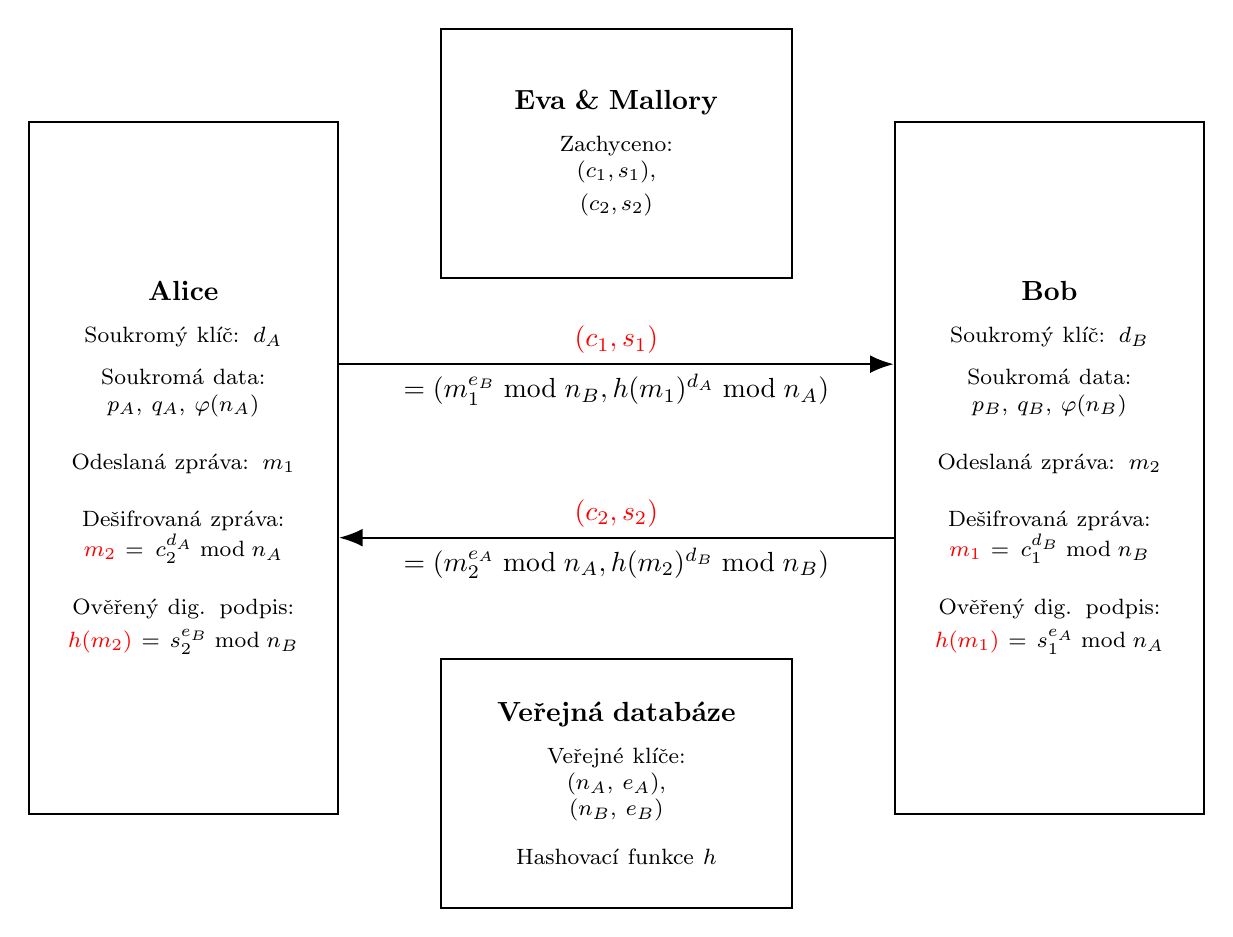
\begin{tikzpicture}[node distance=5cm, thick]

        % Nodes
        \node (A) [rectangle, draw, minimum width=105pt, minimum height=250pt, text centered, text width=105pt] at (0,4)
                    {\textbf{Alice}\\[0.2cm]\footnotesize{Soukromý klíč: $d_A$\\[0.2cm] Soukromá data: \\$p_A$, $q_A$, $\varphi(n_A)$}\\[0.4cm]
                    Odeslaná zpráva: $m_1$\\[0.4cm] Dešifrovaná zpráva:\\\textcolor{red}{$m_2$} $=c_2^{d_A} \bmod{n_A}$\\[0.4cm]
                    Ověřený dig. podpis:\\\textcolor{red}{$h(m_2)$} $=s_2^{e_B} \bmod{n_B}$};

        \node (B) [rectangle, draw, minimum width=105pt, minimum height=250pt, text centered, text width=105pt] at (11,4)
                    {\textbf{Bob}\\[0.2cm]\footnotesize{Soukromý klíč: $d_B$\\[0.2cm] Soukromá data: \\$p_B$, $q_B$, $\varphi(n_B)$}\\[0.4cm]
                    Odeslaná zpráva: $m_2$\\[0.4cm] Dešifrovaná zpráva:\\\textcolor{red}{$m_1$} $=c_1^{d_B} \bmod{n_B}$\\[0.4cm]
                    Ověřený dig. podpis:\\\textcolor{red}{$h(m_1)$} $=s_1^{e_A} \bmod{n_A}$};
        
        \node (P) [rectangle, draw, minimum width=120pt, minimum height=90pt, text centered, text width=120pt] at (5.5,0)
                    {\textbf{Veřejná databáze}\\[0.2cm]\footnotesize{Veřejné klíče: \\$(n_A$, $e_A$),\\$(n_B$, $e_B)$\\[0.2cm] Hashovací funkce $h$}};
        
        \node (E) [rectangle, draw, minimum width=120pt, minimum height=90pt, text centered, text width=120pt] at (5.5, 8)
                    {\textbf{Eva \& Mallory}\\[0.2cm]\footnotesize{
                    Zachyceno:\\
                    $(c_1,s_1)$,\\
                    $(c_2,s_2)$}};
        
        % Arrows
        \draw[-{Latex[length=3mm]}] ($(A.north east)!0.35!(A.south east)$) -- node[midway, above] {\textcolor{red}{$(c_1,s_1)$}} node[midway, below] {$= (m_1^{e_B} \bmod n_B, h(m_1)^{d_A} \bmod{n_A})$} ($(B.north west)!0.35!(B.south west)$);
        \draw[{Latex[length=3mm]}-] ($(A.north east)!0.60!(A.south east)$) -- node[midway, above] {\textcolor{red}{$(c_2,s_2)$}} node[midway, below] {$= (m_2^{e_A} \bmod n_A, h(m_2)^{d_B} \bmod{n_B})$} ($(B.north west)!0.60!(B.south west)$);
        
    \end{tikzpicture}
    \caption{Oboustranná autentizovaná komunikace mezi Alicí a Bobem založená na RSA}\label{fig:RSA-communication}
    \end{figure}

    \newpage


\section{Kryptografie a kvantové počítače}\label{sec:quantum-computers}

    Inspirací pro tuto kapitolu byly díla~\cite{graduate-course} a~\cite{theory-and-practice}.

    Důležitým tématem v kryptografii je vývoj kvantových počítačů a jejich vliv na bezpečnost kryptografických protokolů.
    V této práci jsme uvedli dva významné problémy: problém diskrétního logaritmu (DLP) a problém faktorizace (FP).
    Jejich složitostí vzhledem ke kvantovým počítačům se stručně věnujeme v~následujících sekcích.
    

    \subsection{Kvantové útoky na DLP}\label{sub:quantum-discrete-log}

        Problému DLP a jeho složitosti jsme se detailně věnovali v sekcích~\ref{sub:discrete-log} a~\ref{ss:discrete-log-complexity}.

        O složitost problému DLP se opírá mnoho dalších kryptografických protokolů, mimo jiné
        například Diffieho-Hellmanova výměna klíčů, kterou jsme uvedli i~v~této práci (viz sekce~\ref{sub:diffie-hellman}).
        Konkrétně těžíme z faktu, že neexistuje polynomiální algoritmus, který by DLP řešil.

        Ve světle kvantových počítačů je bezpečnost protokolů, které jsou založeny na~principu DLP, ohrožena.
        Pro problém DLP totiž existuje kvantový algoritmus pracující v polynomiálním čase.
        Tomuto algoritmu se po jeho objeviteli říká \emph{Shorův algoritmus}\footnote{V sekci~\ref{sub:quantum-factoring}
        uvádíme „pravý“ Shorův algoritmus, který řeší problém faktorizace.}.
        Lze ukázat, že tento algoritmus pracuje v čase $O(\log^3{n})$, kde $n$ je řád cyklické grupy, ve které DLP řešíme.


    \subsection{Kvantová faktorizace}\label{sub:quantum-factoring}
        
        Problému FP a jeho složitosti jsme se podrobně věnovali v sekci~\ref{ss:factorization}.
        Uvedli jsme také několik algoritmů, které FP řeší.
        Všechny tyto algoritmy řešili FP buď v exponenciálním čase, nebo neřešili FP obecně (pracovali tedy se specifickým tvarem $n$). 

        O složitost problému FP se opírá mnoho významných protokolů a celých kryptosystémů
        (například RSA z části~\ref{sub:RSA})
        Ty konkrétně využívají faktu, že~dosud není znám polynomiální algoritmus, který by FP řešil.


        S vývojem kvantových počítačů byl ale takový algoritmus objeven.
        Algoritmus je pojmenován po jeho objeviteli: \emph{Shorův algoritmus}.
        Lze ukázat, že časová složitost tohoto algoritmu je $O(\log^3{n})$, kde $n$ je číslo, pro které faktorizaci hledáme.


    \subsection{Postkvantová kryptografie}\label{sub:post-quantum-cryptography}

        Jedinou útěchou může být fakt, že dodnes neexistuje dostatečně efektivní a výkonný kvantový počítač, na kterém
        bychom Shorův algoritmus mohli spustit.\footnote{Respektive dodnes nikdo jeho sestrojení neohlásil.
        Je možné, že někdo takovýmto kvantovým počítačem již disponuje, a jeho sílu využívá tajně pro svou potřebu.}
        Nicméně, v oblasti kvantových počítačů probíhá plynulý vývoj a předpokládá se, že dostatečně výkonný kvantový počítač
        bude sestrojen již v tomto století~\cite{graduate-course}.

        Po přečtení této práce by mělo být jasné, jak výrazné riziko pro bezpečnost kvantové počítače představují.
        Naštěstí pro nás, probíhá i výzkum nových kryptografických systémů, které budou bezpečné i ve světě
        výkonných kvantových počítačů.
        Kryptografii, která bude bezpečná i s příchodem výkonných kvantových počítačů, nazýváme \emph{Postkvantová kryptografie}.
        Spadá do ní například tzv. \emph{mřížková kryptografie}.
        Pro více informací k tématu postkvantové kryptografie čtenáře odkážeme na knihu~\cite{theory-and-practice}.

        \newpage


\section{Eliptické křivky}\label{sec:elliptic-curves}

    Informace pro tuto kapitolu byly čerpány z knihy~\cite{guide-elliptic-curve}.

    V této kapitole se budeme stručně věnovat kryptografii založené na eliptických křivkách.
    Kryptografie eliptických křivek, která pracuje s~cyklickými podgrupami grup eliptických křivek, je svým principem
    velmi podobná té, která pracuje~s cyklickými podgrupami multiplikativních grup (jako to dělá například Diffieho-Hellmanova výměna
    klíčů ze sekce~\ref{sub:diffie-hellman}).
    Bezpečnost kryptografie eliptických křivek bude využívat varianty problému DLP, kterou
    budeme značit ECDLP.\footnote{ECDLP je zkratkou za angl. \emph{elliptic curve discrete log problem}.}.

    \begin{definition}[Eliptická křivka nad $\mathbb{F}_p$]\label{def:elliptic-curve-over-fp}

        Nechť $p$ je prvočíslo a $\mathbb{F}_p$ značí pole zbytkových tříd modulo $p$, kde $p$ je prvočíslo.
        Eliptická křivka $E$ nad $\mathbb{F}_p$ je pak definována rovnicí

            \begin{equation}\label{eq:elliptic-curve}
                y^2 \equiv x^3 + ax + b \pmod{p},
            \end{equation}
              

        \noindent
        kde $a, b \in \mathbb{F}_p$ splňují $4a^3 + 27b^2 \not\equiv 0 \pmod{p}$.
        Páru $(x,y)$, kde $x, y \in \mathbb{F}_p$ se říká \emph{bod na křivce} právě tehdy, když $(x,y)$ splňuje rovnici~(\ref{eq:elliptic-curve}).
        \emph{Bod v nekonečnu}, který se značí jako $\infty$ se také považuje za bod na křivce.
        Množina všech bodů na křivce $E$ nad $\mathbb{F}_p$ se značí $E(\mathbb{F}_p)$.

    \end{definition}

    Binární operaci $\oplus$ nad množinou bodů na křivce říkáme \emph{sčítací pravidlo}.
    Její aplikování se nejlépe popisuje slovně.
    Pro dva body na křivce $P = (x_1,y_1)$ a~$Q = (x_2, y_2)$
    je jejich součet $R = P \oplus Q$ získán následovně:
    
    \begin{itemize}
        \item 
            Sestrojíme přímku vedoucí přes body $P$ a $Q$. Tím získáme třetí průsečík s~křivkou $E$ (označme jej $R'$).
        \item
            $R$ je pak symetrickým obrazem $R'$ vzhledem k ose $x$.
    \end{itemize}

    \begin{remark}
        Pokud $P = Q$, pak je sestrojenou přímkou tečna křivky $E$ v bodě $P$. Operace pak postupuje analogicky.
        Situaci $P \oplus P$ říkáme \emph{zdvojení} bodu $P$.
        Můžeme pak zavést značení $d \cdot P$, čímž myslíme zřetězení $d$ bodů $P$ pomocí operace operace~$\oplus$.
        Tedy například $4 \cdot P = P \oplus P \oplus P \oplus P$.
    \end{remark}

    Operace $\oplus$ je graficky znázorněna na Obrázku~\ref{fig:ec-addition-rule}, který byl převzat z~\cite{guide-elliptic-curve}.

    \begin{figure}
        \centering
        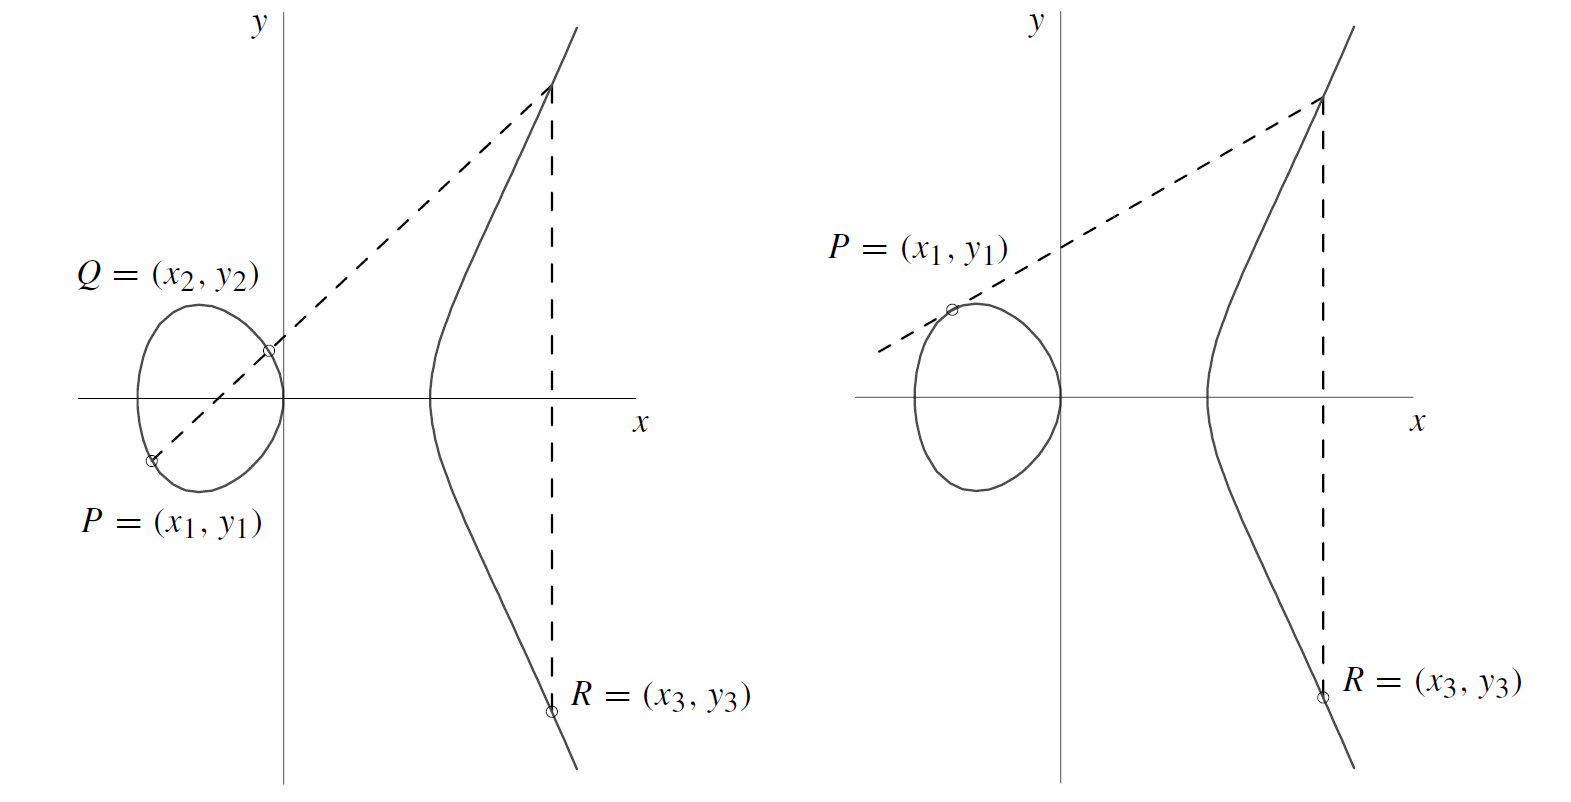
\includegraphics[width=\textwidth]{ec_addition_rule}
        \caption{Grafické znázornění $P \oplus Q$ a zdvojení bodu $P$ na křivce $E_1:y^2 = x^3 - x$ nad $\mathbb{R}$.}\label{fig:ec-addition-rule}
    \end{figure}

    Společně s operací $\oplus$ tvoří množina $E(\mathbb{F}_p)$ abelovskou grupu~\cite{guide-elliptic-curve}.
    Její cyklické podgrupy pak můžeme využít pro implementaci systému založeného na ECDLP.
    Víme, že každá cyklická grupa má generátor.
    Generátor grupy $E(\mathbb{F}_p)$, který je zároveň bodem na křivce, budeme značit $G$.

    Pro demonstraci práce s eliptickými křivkami stručně uvedeme několik algoritmů které eliptické křivky využívají.
    Půjde o algoritmy řešící některé z problémů, kterým jsme se v této práci věnovali.


    \subsection{Diffieho-Hellmanova výměna klíčů s využitím eliptických křivek}

        V části~\ref{sub:diffie-hellman} jsme popsali původní verzi tohoto známého protokolu.
        Uvedli jsme v1~ní také několik důležitých komentářů a myšlenek, které budou platit i pro tuto verzi protokolu.
        Zjednodušený protokol D-H s využitím eliptických křivek bude vypadat následovně:

        Pro funkčnost protokolu potřebujeme, aby Alice i Bob znali generátor $G$ grupy $E(\mathbb{F}_p)$, což.
        není obecně jednoduchý úkol.
        Budeme ale předpokládat, že $G$ (včetně jeho řádu $n$) je parametr sdílený všemi uživateli v síti (i Evou).

        \begin{enumerate}
            \item
                Alice se s Bobem domluví na eliptické křivce $E$ a prvočísle $p$, které určí $\mathbb{F}_p$.
                K~tomu musí Alice poslat Bobovi hodnoty $a, b$ a $p$.
                Nevadí nám, že Eva tyto hodnoty zachytí.
            \item
                Dále se Bob s Alicí musí domluvit na generátoru $G$ grupy $E(\mathbb{F}_p)$.
                Budeme předpokládat, že $G$ (včetně jeho řádu $n$) je parametr sdílený všemi uživateli v síti (i Evou).
            \item
                Alice náhodně vybere číslo $\alpha, 1 \leq \alpha \leq n-1$, vypočítá bod na křivce $A = \alpha \cdot G$ a
                $A = (x_a, y_a)$ pošle po síti Bobovi.
            \item
                Bob náhodně vybere číslo $\beta, 1 \leq \beta \leq n-1$, vypočítá bod na křivce $B = \beta \cdot G$ a
                $B = (x_b, y_b)$ pošle po síti Alici.
            \item
                Alice vypočítá bod $K= \alpha \cdot B = \alpha \beta \cdot G$.
            \item
                Bob vypočítá bod $K= \beta \cdot A = \beta \alpha \cdot G$.

        \end{enumerate}

        Z komutativity násobení plyne, že $\alpha \beta \cdot G = \beta \alpha \cdot G$.
        Z toho vyplývá, že Alice a Bob nezávisle na sobě získají stejný klíč $K = (x_k, y_k)$.\footnote{V praxi
        mohou Alice a Bob jako tajný klíč $k$ použít pouze jednu ze souřadnic bodu $K$.}
        Bezpečnost tohoto protokolu se pak opírá o fakt, že nelze snadno získat hodnotu $\alpha$ z $A = \alpha G$ i se znalostí $G$.
        Tento problém shrnuje následující definice:

        \begin{definition}[Problém diskrétního logaritmu v $E(\mathbb{F}_p)$ (ECDLP)]\label{def:elliptic-curve-dlp}
        
                Nechť $\mathbb{G}$ je cyklická podgrupa $E(\mathbb{F}_p)$ řádu $n$, $G$ její generátor a $Q$ libovolný bod z $G$.
                Číslo $e \in \mathbb{Z}_n$ takové, že
        
                    \begin{equation}\label{eq:elliptic-curve-dlp}
                        e \cdot G = Q.
                    \end{equation}

                \noindent
                nazveme diskrétním logaritmem o základu $G$ z $Q$.
                Nalezení takového čísla $e$ budeme nazývat \textbf{problém diskrétního logaritmu v $E(\mathbb{F}_p)$}.

        \end{definition}

        Podobnost problému DLP a ECDLP je zřejmá.
        To naznačuje, že je operace $\oplus$ vhodnou volbou pro jednosměrnou funkci (viz sekce~\ref{sub:diffie-hellman}).

        Popis protokolu D-H využívajícího eliptické křivky vznikl zjednodušením informací z~\cite{pair-wise-key-establishment}.
        Pro detailnější komentář k obtížnosti ECDLP viz například~\cite{graduate-course} nebo~\cite{guide-elliptic-curve}.


    \subsection{Faktorizace s využitím eliptických křivek (ECM)}

        Komentář k algoritmu ECM byl převzat z knihy~\cite{handbook}.
        Jeho detailní popis lze pak nalézt v knize~\cite{elliptic-curves}.

        Tento faktorizační algoritmus je zobecněním Pollardovy $p-1$ metody, kterou jsme popsali v sekci~\ref{sss:pollard-p-1-method}.
        Ta spoléhala na to, že $p-1$ je $B$-hladké pro nějakého prvočíselného dělitele $p$ čísla $n$.

        Všimněme si, že $p-1$ je řád grupy $\mathbb{Z}^*_p$.
        Algoritmus ECC pak nahradí $\mathbb{Z}^*_p$ náhodnou eliptickou křivkou nad $\mathbb{Z}^*_p$.

        \begin{theorem}
            Časová složitost algoritmu ECM je $\exp{((\sqrt{2} + o(1)) \sqrt{\ln{p} \ln \ln{p}})}$, kde $p$ je \\ nejmenší prvočíselný
            dělitel $n$.
        \end{theorem}

        Vzhledem k tomu, že časová složitost závisí na velikosti prvočíselných dělitelů čísla $n$, je využíván především pro nalezení
        malých prvočíselných dělitelů.

        V případě, kdy $n$ je součinem dvou podobně velkých prvočísel, je časová složitost stejná jako u
        metody kvadratického síta (viz sekce~\ref{sss:quadratic-sieve}).
        Oproti ECC je ale metoda kvadratického síta v praxi efektivnější.
        Může za to typ operací (a~jejich přesnost), které jsou u těchto metod využívány.


    \subsection{Testování prvočíselnosti s využitím eliptických křivek (ECPP)}

        Tento test využívá analogie Pocklingtonovy věty (viz Věta~\ref{the:pocklington}).
        Testu ECPP (z~angl. \emph{Elliptic Curve Primality Proving algorithm}) se někdy také říká \emph{Atkinův test}.

        Výhoda algoritmu ECPP spočívá v připojení krátkého \emph{certifikátu prvočíselnosti} čísla $n$, pomocí
        kterého může uživatel jeho prvočíselnost kdykoli snadno ověřit.

        \begin{theorem}
            Očekávaná časová složitost algoritmu ECPP pro rozhodnutí prvočíselnosti čísla $n$
            je $O((\ln{n})^{6+\epsilon})$ bitových operací, pro libovolné $\epsilon > 0$.
        \end{theorem}
        
        Komentář k algoritmu ECPP byl převzat z~\cite{handbook}.
        Detailní popis algoritmu lze opět nalézt v~\cite{elliptic-curves}.

        \newpage

        


    

\begin{kiconclusions}
    
    V teoretické části této práce jsme se věnovali principům symetrického a asymetrického šifrování.
    Prostor byl věnován také konkrétním šifrám obou typů.
    Několik základních druhů šifer nás poté přimělo definovat konkrétní úrovně bezpečnosti.

    V části o symetrickém šifrování jsme se podrobně věnovali problému diskrétního logaritmu, ke kterému
    nás dovedl popis bezpečnosti Diffieho-Hellmanovy výměny klíčů.
    U problému diskrétního logaritmu jsme popsali vztah jeho obtížnosti s faktorizací a prvočísly.
    Byly také zmíněny konkrétní metody, které problém diskrétního logaritmu řeší.

    V části o asymetrickém šifrování jsme nejprve zmínili rozdíly oproti symetrickému šifrování.
    Konkrétněji jsme prošli možné volby algoritmu zašifrování a generování klíčových párů.
    Následně jsme část práce věnovali třem významným problémům spojeným s prvočísly: problému faktorizace, testování
    prvočíselnosti a generování náhodných prvočísel.
    Uvedli jsme několik algoritmů, které tyto problémy řeší.
    Podrobně jsme pak popsali kryptosystém RSA, jakožto nejvýznamnějšího zástupce asymetrických šifer.
    Zabývali jsme se jeho bezpečností a jeho využitím pro digitální podpisy.

    V závěru práce jsme se stručně věnovali tématu kvantových počítačů a eliptických křivek.
    U kvantových počítačů jsme zmínili rizika spojená s jejich zefektivněním.
    Pro eliptické křivky jsme kromě popisu jejich fungování uvedli varianty algoritmů z této práce, které
    eliptické křivky využívají.

    Jako výstup praktické části byly implementovány vybrané algoritmy řešící problém diskrétního logaritmu a problém faktorizace, společně
    s vybranými testy prvočíselnosti a generátory náhodných prvočísel.

    Práce by se dala zlepšit dodáním detailnějšího popisu vybraných metod faktorizace a testů prvočíselnosti uvedených v této práci.
    Dále bychom mohli práci rozšířit o úvod k teorii složitosti a představit více metod digitálních podpisů.
    Závěrečná dvě témata, kvantové počítače a eliptické křivky, by také zasloužila více prostoru.
    Tato rozšíření by pak mohla práci spojit v uzavřenější a komplexnější celek.
    Praktická část by pak mohla být rozšířena o konzolové rozhraní nasazené na triviální aplikaci, která by
    implementované metody používala. Následně by pak mohlo být přidáno grafické uživatelské rozhraní.

\end{kiconclusions}


\begin{kiconclusions}[english]

    In the theoretical part of this thesis we have discussed the principles of symmetric and asymmetric encryption.
    Space was also devoted to specific ciphers of both types.
    Several basic types of ciphers then led us to define specific levels of security.

    In the section on symmetric encryption, we discussed the discrete logarithm problem, which
    we came across while describing the security of the Diffie-Hellman key exchange.
    For the discrete logarithm problem, we described the relationship of its difficulty with factorization and prime numbers.
    Several methods that solve the discrete logarithm problem were also mentioned.

    In the section on asymmetric encryption, we first mentioned the differences from symmetric encryption.
    More specifically, we went over the possible choices of encryption algorithm and key pair generation.
    We then devoted part of the thesis to three problems associated with prime numbers: the factorization problem, testing
    primality and random prime generation.
    We presented several algorithms that solve these problems.
    We then described the RSA cryptosystem, as the most important asymmetric cipher.
    We discussed its security and its use for digital signatures.

    We briefly concluded the thesis with the topic of quantum computers and elliptic curves.
    For quantum computers, we mentioned the risks associated with the rise of efficient quantum computers.
    For elliptic curves, in addition to describing how they work, we presented variants of the algorithms from this work that use
    elliptic curves.

    As output of the practical part, several algorithms solving the discrete logarithm problem and the factorization problem were implemented, together
    together with several primality tests and random prime generators.

    The work could be improved by providing a more detailed description of the selected factorization methods and primality tests presented in this paper.
    In addition, the thesis could be extended with an introduction to complexity theory and the introduction of more digital signature schemes.
    The final two topics, quantum computers and elliptic curves, also deserved more space.
    These extensions could then bring the work together into a more closed and complex piece.
    The practical part could then be extended with a console UI deployed on a trivial application that would use the
    implemented methods. GUI could then be added.

\end{kiconclusions}


\appendix

\section{Obsah elektronických dat}

\begin{description}

    \item[\texttt{doc/}] \hfill \\
        Text práce ve formátu PDF, vytvořený s~použitím závazného stylu KI
        PřF UP v~Olomouci pro závěrečné práce, včetně všech příloh,
        a~všechny soubory potřebné pro bezproblémové vygenerování PDF
        dokumentu textu, tj.~zdrojový kód textu, vložené
        obrázky, a podobně.
    
    \item[\texttt{docs/}] \hfill \\
    Obsahuje dokumentaci jednotlivých modulů ze složky \textbf{\texttt{impl/}}. Tato dokumentace je přístupná přes soubor \texttt{index.html}.

    \item[\texttt{impl/}] \hfill \\
        Obsahuje moduly zpracovávající jednotlivé problémy probrané v teoretické části,
        modul obsahující uvedené metody kryptosystému RSA a modul, ve kterém je několik příkladů použití
        implementovaných algoritmů a jejich základní testy.

    \item[\texttt{README.txt}] \hfill \\
        Příručka k elektronickým datům práce.
        Obsahuje popis kroků, které je potřeba provést před spuštěním kódu.
      
\end{description}


\begin{thebibliography}{99}

    % APA 7 FOMAT

    \bibitem{rsa-original}
        Rivest, R. L., Shamir, A., \& Adleman, L. (1978).
        A method for obtaining digital signatures and public-key cryptosystems.
        \emph{Communications of the ACM, 21}(2), 120–126.
        \url{https://doi.org/10.1145/359340.359342}

    \bibitem{graduate-course}
        Boneh, D., \& Shoup, V. (2023).
        \emph{A Graduate Course in Applied Cryptography} (ver.~0.6).
        Dostupné z: \url{http://toc.cryptobook.us/}

    \bibitem{theory-and-practice}
        Stinson, D. R., \& Paterson, M. B. (2018).
        \emph{Cryptography: Theory and Practice} (ed.~4).
        Chapman and Hall/CRC.
        ISBN~978-1138197015.

    \bibitem{computational-introduction}
        Shoup, V. (2009).
        \emph{A Computational Introduction to Number Theory and Algebra} (ver.~2).
        Dostupné z: \url{https://www.shoup.net/ntb/}

    \bibitem{rsa-and-public}
        Mollin, R. A. (2002).
        \emph{RSA and Public-Key Cryptography} (ed.~1).
        Chapman and Hall/CRC.
        ISBN~1-58488-338-3.

    \bibitem{foundations-cryptography}
        Goldreich, O. (2004)
        \emph{Foundations of Cryptography: Basic Techniques} (ed.~1).
        Cambridge University Press.
        ISBN~0-511-04120-9.

    \bibitem{complexity}
        Immerman, N. (1998).
        \emph{Descriptive Complexity}.
        Springer Science \& Business Media.
        ISBN~978-0-387-98600-5.

    \bibitem{comparison-dlp-factorization}
        Van Oorschot, P. C. (1990).
        A Comparison of Practical Public-Key Cryptosystems based on Integer Factorization and Discrete Logarithms.
        \emph{Lecture Notes in Computer Science}.
        \url{https://doi.org/10.1007/3-540-38424-3_40}

    \bibitem{handbook}
        Menezes, A. J., Van Oorschot, P. C., \& Vanstone, S. A. (1997)
        \emph{Handbook of Applied Cryptography}.
        CRC Press.
        ISBN~0-8493-8523-7.
        Jednotlivé kapitoly dostupné z: \url{https://cacr.uwaterloo.ca/hac/}

    \bibitem{primes-and-factorization}
        Riesel, H. (2011).
        \emph{Prime Numbers and Computer Methods for Factorization} (ed.~2).
        Birkhäuser.
        ISBN~978-0-8176-8297-2.

    \bibitem{method-p+1}
        Williams, H.C. (1982).
        A $p+1$ method of factoring.
        \emph{Mathematics of Computation, 39}(159), 225--234.
        \url{https://doi.org/10.1090/s0025-5718-1982-0658227-7}.

    \bibitem{squfof-implementation}
        Gower, J. E., \& Wagstaff, S. S. (2008).
        Square form factorization.
        \emph{Mathematics of Computation, 77}(261), 551–588.
        \url{https://doi.org/10.1090/s0025-5718-07-02010-8}
        Dostupné z: \url{https://homes.cerias.purdue.edu/~ssw/squfof.pdf}

    \bibitem{primes-in-p}
        Agrawal, M., Kayal, N., \& Saxena, N. (2004).
        PRIMES is in P.
        \emph{Annals of Mathematics, 160}(2), 781–793.
        \url{https://doi.org/10.4007/annals.2004.160.781}

    \bibitem{20-years-attacks}
        Boneh, D. (1999).
        Twenty Years of Attacks on the RSA Cryptosystem.
        \emph{Notices of the American Mathematical Society, 46}(2), 203--213.
        Dostupné z: \url{https://www.ams.org/notices/199902/199902FullIssue.pdf}

    \bibitem{optimal-asymmetric-encryption}
        Bellare, M., \& Rogaway, P. (1994).
        Optimal asymmetric encryption.
        \emph{Lecture Notes in Computer Science}, 92–-111
        \url{https://doi.org/10.1007/bfb0053428}

    \bibitem{guide-elliptic-curve}
        Hankerson, D., Menezes, A. J., \& Vanstone, S. (2004)
        \emph{Guide to Elliptic Curve Cryptography.}
        Springer Science \& Business Media.
        ISBN~0-387-95273-X.

    \bibitem{pair-wise-key-establishment}
        Barker, E., Chen, L., Roginsky, A., Vassilev, A., \& Davis, R. (2018).
        Recommendation for pair-wise key-establishment schemes using discrete logarithm cryptography.
        \emph{Journal of Research of NIST}.
        \url{https://doi.org/10.6028/nist.sp.800-56ar3}

    \bibitem{elliptic-curves}
        Husemöller, D. (2004).
        \emph{Elliptic Curves} (ed.~2).
        Springer Science \& Business Media.
        ISBN~0-387-95490-2.

    

\end{thebibliography}

\end{document}